%&preformat-disser
\RequirePackage[l2tabu,orthodox]{nag}
% Формат А4, 14pt (ГОСТ Р 7.0.11-2011, 5.3.6)
\documentclass[a4paper,14pt,oneside,openany]{memoir}

\input{common/setup}            % общие настройки шаблона
%%% Проверка используемого TeX-движка %%%
\RequirePackage{ifxetex, ifluatex}
\newif\ifxetexorluatex   % определяем новый условный оператор (http://tex.stackexchange.com/a/47579)
\ifxetex
    \xetexorluatextrue
\else
    \ifluatex
        \xetexorluatextrue
    \else
        \xetexorluatexfalse
    \fi
\fi

\newif\ifsynopsis           % Условие, проверяющее, что документ --- автореферат

\RequirePackage{etoolbox}[2015/08/02]               % Для продвинутой проверки разных условий
\providebool{presentation}

\usepackage{cite}
\usepackage[resetlabels]{multibib}
\newcites{author}{References}

%%% Поля и разметка страницы %%%
\usepackage{pdflscape}                              % Для включения альбомных страниц
\usepackage{geometry}                               % Для последующего задания полей

%%% Математические пакеты %%%
\usepackage[overload]{empheq}
\usepackage{amsthm,amsmath,amscd}   % Математические дополнения от AMS
\usepackage{amsfonts,amssymb}       % Математические дополнения от AMS
\usepackage{mathtools}              % Добавляет окружение multlined

%%%% Установки для размера шрифта 14 pt %%%%
%% Формирование переменных и констант для сравнения (один раз для всех подключаемых файлов)%%
%% должно располагаться до вызова пакета fontspec или polyglossia, потому что они сбивают его работу
\newlength{\curtextsize}
\newlength{\bigtextsize}
\setlength{\bigtextsize}{13.9pt}

\makeatletter
%\show\f@size                                       % неплохо для отслеживания, но вызывает стопорение процесса, если документ компилируется без команды  -interaction=nonstopmode
\setlength{\curtextsize}{\f@size pt}
\makeatother

%%% Кодировки и шрифты %%%
\ifxetexorluatex
    \usepackage{polyglossia}[2014/05/21]            % Поддержка многоязычности (fontspec подгружается автоматически)
\else
   %%% Решение проблемы копирования текста в буфер кракозябрами
    \ifnumequal{\value{usealtfont}}{0}{}{
        \input glyphtounicode.tex
        \input glyphtounicode-cmr.tex %from pdfx package
        \pdfgentounicode=1
    }
    \usepackage{cmap}                               % Улучшенный поиск русских слов в полученном pdf-файле
    \ifnumequal{\value{usealtfont}}{2}{}{
        \defaulthyphenchar=127                      % Если стоит до fontenc, то переносы не впишутся в выделяемый текст при копировании его в буфер обмена
    }
    \usepackage{textcomp}
    \usepackage[T1,T2A]{fontenc}                    % Поддержка русских букв
    \ifnumequal{\value{usealtfont}}{1}{% Используется pscyr, при наличии
        \IfFileExists{pscyr.sty}{\usepackage{pscyr}}{}  % Подключение pscyr
    }{}
    \usepackage[utf8]{inputenc}[2014/04/30]         % Кодировка utf8
    \usepackage[english, russian]{babel}[2014/03/24]% Языки: русский, английский
    \ifnumequal{\value{usealtfont}}{2}{
        % http://dxdy.ru/post1238763.html#p1238763
        \usepackage[scaled=0.960]{XCharter}[2017/12/19] % Подключение русифицированных шрифтов XCharter
        \usepackage[charter, vvarbb, scaled=1.048]{newtxmath}[2017/12/14]
        \setDisplayskipStretch{-0.078}
    }{}
\fi

%%% Оформление абзацев %%%
\usepackage{indentfirst}                            % Красная строка

%%% Цвета %%%
\ifpresentation
\else
    \usepackage[dvipsnames, table, hyperref]{xcolor} % Совместимо с tikz
\fi

%%% Таблицы %%%
%\usepackage{longtable,ltcaption}                    % Длинные таблицы
\usepackage{longtable}
\usepackage{tabularx}
\usepackage{caption}
\usepackage{multirow,makecell}                      % Улучшенное форматирование таблиц

%%% Общее форматирование
\usepackage{soulutf8}                               % Поддержка переносоустойчивых подчёркиваний и зачёркиваний
\usepackage{icomma}                                 % Запятая в десятичных дробях

%%% Оптимизация расстановки переносов и длины последней строки абзаца
\ifluatex
    \ifnumequal{\value{draft}}{1}{% Черновик
        \usepackage[hyphenation, lastparline, nosingleletter, homeoarchy,
        rivers, draft]{impnattypo}
    }{% Чистовик
        \usepackage[hyphenation, lastparline, nosingleletter]{impnattypo}
    }
\else
    \usepackage[hyphenation, lastparline]{impnattypo}
\fi

%%% Гиперссылки %%%
\usepackage{hyperref}[2012/11/06]

%%% Изображения %%%
\usepackage{graphicx}[2014/04/25]                   % Подключаем пакет работы с графикой

%%% Счётчики %%%
\usepackage[figure,table]{totalcount}               % Счётчик рисунков и таблиц
\usepackage{totcount}                               % Пакет создания счётчиков на основе последнего номера подсчитываемого элемента (может требовать дважды компилировать документ)
\usepackage{totpages}                               % Счётчик страниц, совместимый с hyperref (ссылается на номер последней страницы). Желательно ставить последним пакетом в преамбуле

\usepackage{pgfplots}
\usepackage{pgfplotstable}
\usepackage{wrapfig}
\usepackage{colortbl}
\usepackage{tikz}

%%% Продвинутое управление групповыми ссылками (пока только формулами) %%%
\ifpresentation
\else
    \ifxetexorluatex
        \usepackage{cleveref}                           % cleveref корректно считывает язык из настроек polyglossia
    \else
        \usepackage[russian]{cleveref}                  % cleveref имеет сложности со считыванием языка из babel. Такое решение русификации вывода выбрано вместо определения в documentclass из опасности что-то лишнее передать во все остальные пакеты, включая библиографию.
    \fi
    \creflabelformat{equation}{#2#1#3}                  % Формат по умолчанию ставил круглые скобки вокруг каждого номера ссылки, теперь просто номера ссылок без какого-либо дополнительного оформления
    \crefrangelabelformat{equation}{#3#1#4\cyrdash#5#2#6}   % Интервалы в русском языке принято делать через тире, если иное не оговорено
\fi

\ifnumequal{\value{draft}}{1}{% Черновик
    \usepackage[firstpage]{draftwatermark}
    \SetWatermarkText{DRAFT}
    \SetWatermarkFontSize{14pt}
    \SetWatermarkScale{15}
    \SetWatermarkAngle{45}
}{}

%%% Исправление положения якорей подписей (под)рисунков %%%
% Без hypcap и патча, при клике по ссылке на подрисунок, просмотрщик pdf прыгает "к подписи" а не "к рисунку".
% Подробнее: https://github.com/AndreyAkinshin/Russian-Phd-LaTeX-Dissertation-Template/issues/238
% (!) Даже с патчем, если мешать в одной фиге разные типы подфиг (subbottom и subcaption) - ссылки всё равно будут работать неправильно  (см. https://www.overleaf.com/read/czmbmmtnqrrg ).
\ifpresentation
\else
    \usepackage[all]{hypcap}

    \makeatletter
    \ltx@ifclasslater{memoir}{2018/12/13}{
        % Предполагается, что в следующей версии класс будет исправлен
        \typeout{Assuming this version of memoir is free from the jumping-to-caption bug.}
    }{
        \RequirePackage{xpatch}

        \newcommand\mem@step@subcounter{\refstepcounter{sub\@captype}\@contkeep}

        \xpatchcmd{\@memsubbody}%
        {\refstepcounter{sub\@captype}\@contkeep}% search pattern
        {}% replacement
        {\typeout{@memsubbody is patched}}%
        {\typeout{@memsubbody is NOT patched}}%

        \xpatchcmd{\@memcontsubbody}%
        {\refstepcounter{sub\@captype}\@contkeep}% pattern
        {}% replacement
        {\typeout{@memcontsubbody is patched}}%
        {\typeout{@memcontsubbody is NOT patched}}%

        \xpatchcmd{\@memsubfloat}%
        {\vbox\bgroup}% search pattern
        {\vbox\bgroup\mem@step@subcounter}% replacement
        {\typeout{@memsubfloat patch is ok}}%
        {\typeout{@memsubfloat patch is NOT ok}}%

        \xpatchcmd{\subcaption}%
        {\refstepcounter{sub\@captype}}% search pattern
        {\H@refstepcounter{sub\@captype}}% replacement
        {\typeout{subcaption second patch is ok}}%
        {\typeout{subcaption second patch is NOT ok}}%
    }
    \makeatother
\fi

%%% Цитата, не приводимая в автореферате:
% возможно, актуальна только для biblatex
%\newcommand{\citeinsynopsis}[1]{\ifsynopsis\else ~\cite{#1} \fi}
         % Пакеты общие для диссертации и автореферата
\synopsisfalse                      % Этот документ --- не автореферат
\input{Dissertation/dispackages}    % Пакеты для диссертации
\input{Dissertation/userpackages}   % Пакеты для специфических пользовательских задач

\input{Dissertation/setup}      % Упрощённые настройки шаблона

\input{common/newnames}         % Новые переменные, для всего проекта

%%% Основные сведения %%%
\newcommand{\thesisAuthorLastName}{Люпа}
\newcommand{\thesisAuthorOtherNames}{Анастасия Александровна}
\newcommand{\thesisAuthorInitials}{А.\,А.}
\newcommand{\thesisAuthor}             % Диссертация, ФИО автора
{%
    \texorpdfstring{% \texorpdfstring takes two arguments and uses the first for (La)TeX and the second for pdf
        \thesisAuthorLastName~\thesisAuthorOtherNames% так будет отображаться на титульном листе или в тексте, где будет использоваться переменная
    }{%
        \thesisAuthorLastName, \thesisAuthorOtherNames% эта запись для свойств pdf-файла. В таком виде, если pdf будет обработан программами для сбора библиографических сведений, будет правильно представлена фамилия.
    }
}
\newcommand{\thesisAuthorShort}        % Диссертация, ФИО автора инициалами
{\thesisAuthorInitials~\thesisAuthorLastName}
%\newcommand{\thesisUdk}                % Диссертация, УДК
%{\todo{xxx.xxx}}
\newcommand{\thesisTitle}              % Диссертация, название
{<<Разработка и анализ вычислительных алгоритмов явного типа для моделирования процессов многофазной фильтрации>>}
\newcommand{\thesisSpecialtyNumber}    % Диссертация, специальность, номер
{09.06.01}
\newcommand{\thesisSpecialtyTitle}     % Диссертация, специальность, название (название взято с сайта ВАК для примера)
{Информатика и вычислительная техника}
\newcommand{\thesisSpecialtyTwoNumber} % Диссертация, вторая специальность, номер
{05.13.18}
\newcommand{\thesisSpecialtyTwoTitle}  % Диссертация, вторая специальность, название
 {Математическое моделирование, численные методы и комплексы программ}
\newcommand{\thesisDegree}             % Диссертация, ученая степень
{\todo{кандидата физико-математических наук}}
\newcommand{\thesisDegreeShort}        % Диссертация, ученая степень, краткая запись
{\todo{канд. физ.-мат. наук}}
\newcommand{\thesisCity}               % Диссертация, город написания диссертации
{Москва}
\newcommand{\thesisYear}               % Диссертация, год написания диссертации
{2019}
\newcommand{\thesisOrganization}       % Диссертация, организация
{Федеральное государственное автономное образовательное учреждение высшего
образования <<Московский физико-технический институт (государственный университет)>>}
\newcommand{\thesisOrganizationShort}  % Диссертация, краткое название организации для доклада
{МФТИ(ГУ)}

\newcommand{\thesisInOrganization}     % Диссертация, организация в предложном падеже: Работа выполнена в ...
{\todo{учреждении с~длинным длинным длинным длинным названием, в~котором
выполнялась данная диссертационная работа}}

\newcommand{\supervisorFio}              % Научный руководитель, ФИО
{Четверушкин Борис Николаевич}
\newcommand{\supervisorRegalia}          % Научный руководитель, регалии
{д.ф.-м.н., профессор, академик РАН}
\newcommand{\supervisorFioShort}         % Научный руководитель, ФИО
{Б.\,Н.~Четверушкин}
\newcommand{\supervisorRegaliaShort}     % Научный руководитель, регалии
{д.ф.-м.н., профессор, академик РАН}

\newcommand{\opponentOneFio}           % Оппонент 1, ФИО
{\todo{Фамилия Имя Отчество}}
\newcommand{\opponentOneRegalia}       % Оппонент 1, регалии
{\todo{доктор физико-математических наук, профессор}}
\newcommand{\opponentOneJobPlace}      % Оппонент 1, место работы
{\todo{Не очень длинное название для места работы}}
\newcommand{\opponentOneJobPost}       % Оппонент 1, должность
{\todo{старший научный сотрудник}}

\newcommand{\opponentTwoFio}           % Оппонент 2, ФИО
{\todo{Фамилия Имя Отчество}}
\newcommand{\opponentTwoRegalia}       % Оппонент 2, регалии
{\todo{кандидат физико-математических наук}}
\newcommand{\opponentTwoJobPlace}      % Оппонент 2, место работы
{\todo{Основное место работы c длинным длинным длинным длинным названием}}
\newcommand{\opponentTwoJobPost}       % Оппонент 2, должность
{\todo{старший научный сотрудник}}

\newcommand{\leadingOrganizationTitle} % Ведущая организация, дополнительные строки. Удалить, чтобы не отображать в автореферате
{\todo{Федеральное государственное бюджетное образовательное учреждение высшего
профессионального образования с~длинным длинным длинным длинным названием}}

\newcommand{\defenseDate}              % Защита, дата
{\todo{DD mmmmmmmm YYYY~г.~в~XX часов}}
\newcommand{\defenseCouncilNumber}     % Защита, номер диссертационного совета
{\todo{Д\,123.456.78}}
\newcommand{\defenseCouncilTitle}      % Защита, учреждение диссертационного совета
{\todo{Название учреждения}}
\newcommand{\defenseCouncilAddress}    % Защита, адрес учреждение диссертационного совета
{\todo{Адрес}}
\newcommand{\defenseCouncilPhone}      % Телефон для справок
{\todo{+7~(0000)~00-00-00}}

\newcommand{\defenseSecretaryFio}      % Секретарь диссертационного совета, ФИО
{\todo{Фамилия Имя Отчество}}
\newcommand{\defenseSecretaryRegalia}  % Секретарь диссертационного совета, регалии
{\todo{д-р~физ.-мат. наук}}            % Для сокращений есть ГОСТы, например: ГОСТ Р 7.0.12-2011 + http://base.garant.ru/179724/#block_30000

\newcommand{\synopsisLibrary}          % Автореферат, название библиотеки
{\todo{Название библиотеки}}
\newcommand{\synopsisDate}             % Автореферат, дата рассылки
{\todo{DD mmmmmmmm YYYY года}}

% To avoid conflict with beamer class use \providecommand
\providecommand{\keywords}%            % Ключевые слова для метаданных PDF диссертации и автореферата
{}
             % Основные сведения
\input{common/fonts}            % Определение шрифтов (частичное)
%%% Шаблон %%%
\DeclareRobustCommand{\todo}{\textcolor{red}}       % решаем проблему превращения названия цвета в результате \MakeUppercase, http://tex.stackexchange.com/a/187930, \DeclareRobustCommand protects \todo from expanding inside \MakeUppercase
\AtBeginDocument{%
    \setlength{\parindent}{2.5em}                   % Абзацный отступ. Должен быть одинаковым по всему тексту и равен пяти знакам (ГОСТ Р 7.0.11-2011, 5.3.7).
}

%%% Подписи %%%
\setlength{\abovecaptionskip}{0pt}   % Отбивка над подписью
\setlength{\belowcaptionskip}{0pt}   % Отбивка под подписью
%\captionwidth{\linewidth}
%\normalcaptionwidth

%%% Таблицы %%%
\ifnumequal{\value{tabcap}}{0}{%
    \newcommand{\tabcapalign}{\raggedright}  % по левому краю страницы или аналога parbox
    \renewcommand{\tablabelsep}{~\cyrdash\ } % тире как разделитель идентификатора с номером от наименования
    \newcommand{\tabtitalign}{}
}{%
    \ifnumequal{\value{tablaba}}{0}{%
        \newcommand{\tabcapalign}{\raggedright}  % по левому краю страницы или аналога parbox
    }{}

    \ifnumequal{\value{tablaba}}{1}{%
        \newcommand{\tabcapalign}{\centering}    % по центру страницы или аналога parbox
    }{}

    \ifnumequal{\value{tablaba}}{2}{%
        \newcommand{\tabcapalign}{\raggedleft}   % по правому краю страницы или аналога parbox
    }{}

    \ifnumequal{\value{tabtita}}{0}{%
        \newcommand{\tabtitalign}{\par\raggedright}  % по левому краю страницы или аналога parbox
    }{}

    \ifnumequal{\value{tabtita}}{1}{%
        \newcommand{\tabtitalign}{\par\centering}    % по центру страницы или аналога parbox
    }{}

    \ifnumequal{\value{tabtita}}{2}{%
        \newcommand{\tabtitalign}{\par\raggedleft}   % по правому краю страницы или аналога parbox
    }{}
}

\precaption{\tabcapalign} % всегда идет перед подписью или \legend
\captionnamefont{\normalfont\normalsize} % Шрифт надписи «Таблица #»; также определяет шрифт у \legend
\captiondelim{\tablabelsep} % разделитель идентификатора с номером от наименования
\captionstyle[\tabtitalign]{\tabtitalign}
\captiontitlefont{\normalfont\normalsize} % Шрифт с текстом подписи

%%% Рисунки %%%
\setfloatadjustment{figure}{%
    \setlength{\abovecaptionskip}{0pt}   % Отбивка над подписью
    \setlength{\belowcaptionskip}{0pt}   % Отбивка под подписью
    \precaption{} % всегда идет перед подписью или \legend
    \captionnamefont{\normalfont\normalsize} % Шрифт надписи «Рисунок #»; также определяет шрифт у \legend
    \captiondelim{\figlabelsep} % разделитель идентификатора с номером от наименования
    \captionstyle[\centering]{\centering} % Центрирование подписей, заданных командой \caption и \legend
    \captiontitlefont{\normalfont\normalsize} % Шрифт с текстом подписи
    \postcaption{} % всегда идет после подписи или \legend, и с новой строки
}

%%% Подписи подрисунков %%%
\newsubfloat{figure} % Включает возможность использовать подрисунки у окружений figure
\renewcommand{\thesubfigure}{\asbuk{subfigure}}           % Буквенные номера подрисунков
\subcaptionsize{\normalsize} % Шрифт подписи названий подрисунков (не отличается от основного)
\subcaptionlabelfont{\normalfont}
\subcaptionfont{\!\!) \normalfont} % Вот так тут добавили скобку после буквы.
\subcaptionstyle{\centering}
%\subcaptionsize{\fontsize{12pt}{13pt}\selectfont} % объявляем шрифт 12pt для использования в подписях, тут же надо интерлиньяж объявлять, если не наследуется

%%% Настройки гиперссылок %%%
\ifluatex
    \hypersetup{
        unicode,                % Unicode encoded PDF strings
    }
\fi

\hypersetup{
    linktocpage=true,           % ссылки с номера страницы в оглавлении, списке таблиц и списке рисунков
%    linktoc=all,                % both the section and page part are links
%    pdfpagelabels=false,        % set PDF page labels (true|false)
    plainpages=false,           % Forces page anchors to be named by the Arabic form  of the page number, rather than the formatted form
    colorlinks,                 % ссылки отображаются раскрашенным текстом, а не раскрашенным прямоугольником, вокруг текста
    linkcolor={linkcolor},      % цвет ссылок типа ref, eqref и подобных
    citecolor={citecolor},      % цвет ссылок-цитат
    urlcolor={urlcolor},        % цвет гиперссылок
%    hidelinks,                  % Hide links (removing color and border)
    pdftitle={\thesisTitle},    % Заголовок
    pdfauthor={\thesisAuthor},  % Автор
    pdfsubject={\thesisSpecialtyNumber\ \thesisSpecialtyTitle},      % Тема
%    pdfcreator={Создатель},     % Создатель, Приложение
%    pdfproducer={Производитель},% Производитель, Производитель PDF
    pdfkeywords={\keywords},    % Ключевые слова
    pdflang={ru},
}
\ifnumequal{\value{draft}}{1}{% Черновик
    \hypersetup{
        draft,
    }
}{}

%%% Списки %%%
% Используем короткое тире (endash) для ненумерованных списков (ГОСТ 2.105-95, пункт 4.1.7, требует дефиса, но так лучше смотрится)
\renewcommand{\labelitemi}{\normalfont\bfseries{--}}

% Перечисление строчными буквами латинского алфавита (ГОСТ 2.105-95, 4.1.7)
%\renewcommand{\theenumi}{\alph{enumi}}
%\renewcommand{\labelenumi}{\theenumi)}

% Перечисление строчными буквами русского алфавита (ГОСТ 2.105-95, 4.1.7)
\makeatletter
\AddEnumerateCounter{\asbuk}{\russian@alph}{щ}      % Управляем списками/перечислениями через пакет enumitem, а он 'не знает' про asbuk, потому 'учим' его
\makeatother
%\renewcommand{\theenumi}{\asbuk{enumi}} %первый уровень нумерации
%\renewcommand{\labelenumi}{\theenumi)} %первый уровень нумерации
\renewcommand{\theenumii}{\asbuk{enumii}} %второй уровень нумерации
\renewcommand{\labelenumii}{\theenumii)} %второй уровень нумерации
\renewcommand{\theenumiii}{\arabic{enumiii}} %третий уровень нумерации
\renewcommand{\labelenumiii}{\theenumiii)} %третий уровень нумерации

\setlist{nosep,%                                    % Единый стиль для всех списков (пакет enumitem), без дополнительных интервалов.
    labelindent=\parindent,leftmargin=*%            % Каждый пункт, подпункт и перечисление записывают с абзацного отступа (ГОСТ 2.105-95, 4.1.8)
}
           % Стили общие для диссертации и автореферата
%%% Переопределение именований, если иначе не сработает %%%
%\gappto\captionsrussian{
%    \renewcommand{\chaptername}{Глава}
%    \renewcommand{\appendixname}{Приложение} % (ГОСТ Р 7.0.11-2011, 5.7)
%}

%%% Изображения %%%
\graphicspath{{images/}{Dissertation/images/}}         % Пути к изображениям

%%% Интервалы %%%
%% По ГОСТ Р 7.0.11-2011, пункту 5.3.6 требуется полуторный интервал
%% Реализация средствами класса (на основе setspace) ближе к типографской классике.
%% И правит сразу и в таблицах (если со звёздочкой)
%\DoubleSpacing*     % Двойной интервал
\OnehalfSpacing*    % Полуторный интервал
%\setSpacing{1.42}   % Полуторный интервал, подобный Ворду (возможно, стоит включать вместе с предыдущей строкой)

%%% Макет страницы %%%
% Выставляем значения полей (ГОСТ 7.0.11-2011, 5.3.7)
\geometry{a4paper, top=2cm, bottom=2cm, left=2.5cm, right=1cm, nofoot, nomarginpar} %, heightrounded, showframe
\setlength{\topskip}{0pt}   %размер дополнительного верхнего поля
\setlength{\footskip}{12.3pt} % снимет warning, согласно https://tex.stackexchange.com/a/334346

%%% Выравнивание и переносы %%%
%% http://tex.stackexchange.com/questions/241343/what-is-the-meaning-of-fussy-sloppy-emergencystretch-tolerance-hbadness
%% http://www.latex-community.org/forum/viewtopic.php?p=70342#p70342
\tolerance 1414
\hbadness 1414
\emergencystretch 1.5em % В случае проблем регулировать в первую очередь
\hfuzz 0.3pt
\vfuzz \hfuzz
%\raggedbottom
%\sloppy                 % Избавляемся от переполнений
\clubpenalty=10000      % Запрещаем разрыв страницы после первой строки абзаца
\widowpenalty=10000     % Запрещаем разрыв страницы после последней строки абзаца
\brokenpenalty=4991     % Ограничение на разрыв страницы, если строка заканчивается переносом
\parindent=1.25cm

%%% Блок управления параметрами для выравнивания заголовков в тексте %%%
\newlength{\otstuplen}
\setlength{\otstuplen}{\theotstup\parindent}
\ifnumequal{\value{headingalign}}{0}{% выравнивание заголовков в тексте
    \newcommand{\hdngalign}{\centering}                % по центру
    \newcommand{\hdngaligni}{}% по центру
    \setlength{\otstuplen}{0pt}
}{%
    \newcommand{\hdngalign}{}                 % по левому краю
    \newcommand{\hdngaligni}{\hspace{\otstuplen}}      % по левому краю
} % В обоих случаях вроде бы без переноса, как и надо (ГОСТ Р 7.0.11-2011, 5.3.5)

%%% Оглавление %%%
\renewcommand{\cftchapterdotsep}{\cftdotsep}                % отбивка точками до номера страницы начала главы/раздела

%% Переносить слова в заголовке не допускается (ГОСТ Р 7.0.11-2011, 5.3.5). Заголовки в оглавлении должны точно повторять заголовки в тексте (ГОСТ Р 7.0.11-2011, 5.2.3). Прямого указания на запрет переносов в оглавлении нет, но по той же логике невнесения искажений в смысл, лучше в оглавлении не переносить:
\setrmarg{2.55em plus1fil}                             %To have the (sectional) titles in the ToC, etc., typeset ragged right with no hyphenation
\renewcommand{\cftchapterpagefont}{\normalfont}        % нежирные номера страниц у глав в оглавлении
\renewcommand{\cftchapterleader}{\cftdotfill{\cftchapterdotsep}}% нежирные точки до номеров страниц у глав в оглавлении
%\renewcommand{\cftchapterfont}{}                       % нежирные названия глав в оглавлении

\ifnumgreater{\value{headingdelim}}{0}{%
    \renewcommand\cftchapteraftersnum{.\space}       % добавляет точку с пробелом после номера раздела в оглавлении
}{}
\ifnumgreater{\value{headingdelim}}{1}{%
    \renewcommand\cftsectionaftersnum{.\space}       % добавляет точку с пробелом после номера подраздела в оглавлении
    \renewcommand\cftsubsectionaftersnum{.\space}    % добавляет точку с пробелом после номера подподраздела в оглавлении
    \renewcommand\cftsubsubsectionaftersnum{.\space} % добавляет точку с пробелом после номера подподподраздела в оглавлении
    \AtBeginDocument{% без этого polyglossia сама всё переопределяет
        \setsecnumformat{\csname the#1\endcsname.\space}
    }
}{%
    \AtBeginDocument{% без этого polyglossia сама всё переопределяет
        \setsecnumformat{\csname the#1\endcsname\quad}
    }
}

\renewcommand*{\cftappendixname}{\appendixname\space} % Слово Приложение в оглавлении

%%% Колонтитулы %%%
% Порядковый номер страницы печатают на середине верхнего поля страницы (ГОСТ Р 7.0.11-2011, 5.3.8)
\makeevenhead{plain}{}{\thepage}{}
\makeoddhead{plain}{}{\thepage}{}
\makeevenfoot{plain}{}{}{}
\makeoddfoot{plain}{}{}{}
\pagestyle{plain}

%%% добавить Стр. над номерами страниц в оглавлении
%%% http://tex.stackexchange.com/a/306950
\newif\ifendTOC

\newcommand*{\tocheader}{
\ifnumequal{\value{pgnum}}{1}{%
    \ifendTOC\else\hbox to \linewidth%
      {\noindent{}~\hfill{Стр.}}\par%
      \ifnumless{\value{page}}{3}{}{%
        \vspace{0.5\onelineskip}
      }
      \afterpage{\tocheader}
    \fi%
}{}%
}%

%%% Оформление заголовков глав, разделов, подразделов %%%
%% Работа должна быть выполнена ... размером шрифта 12-14 пунктов (ГОСТ Р 7.0.11-2011, 5.3.8). То есть не должно быть надписей шрифтом более 14. Так и поставим.
%% Эти установки будут давать одинаковый результат независимо от выбора базовым шрифтом 12 пт или 14 пт
\newcommand{\basegostsectionfont}{\fontsize{14pt}{14pt}\selectfont\bfseries}

\makechapterstyle{thesisgost}{%
    \chapterstyle{default}
    \setlength{\beforechapskip}{0pt}
    \setlength{\midchapskip}{0pt}
    \setlength{\afterchapskip}{\theintvl\curtextsize}
    \renewcommand*{\chapnamefont}{\basegostsectionfont}
    \renewcommand*{\chapnumfont}{\basegostsectionfont}
    \renewcommand*{\chaptitlefont}{\basegostsectionfont}
    \renewcommand*{\chapterheadstart}{}
    \ifnumgreater{\value{headingdelim}}{0}{%
        \renewcommand*{\afterchapternum}{.\space}   % добавляет точку с пробелом после номера раздела
    }{%
        \renewcommand*{\afterchapternum}{\quad}     % добавляет \quad после номера раздела
    }
    \renewcommand*{\printchapternum}{\hdngaligni\hdngalign\chapnumfont \thechapter}
    \renewcommand*{\printchaptername}{}
    \renewcommand*{\printchapternonum}{\hdngaligni\hdngalign}
}

\makeatletter
\makechapterstyle{thesisgostchapname}{%
    \chapterstyle{thesisgost}
    \renewcommand*{\printchapternum}{\chapnumfont \thechapter}
    \renewcommand*{\printchaptername}{\hdngaligni\hdngalign\chapnamefont \@chapapp} %
}
\makeatother

\chapterstyle{thesisgost}

\setsecheadstyle{\basegostsectionfont\hdngalign}
\setsecindent{\otstuplen}

\setsubsecheadstyle{\basegostsectionfont\hdngalign}
\setsubsecindent{\otstuplen}

\setsubsubsecheadstyle{\basegostsectionfont\hdngalign}
\setsubsubsecindent{\otstuplen}

\sethangfrom{\noindent #1} %все заголовки подразделов центрируются с учетом номера, как block

\ifnumequal{\value{chapstyle}}{1}{%
    \chapterstyle{thesisgostchapname}
    \renewcommand*{\cftchaptername}{\chaptername\space} % будет вписано слово Глава перед каждым номером раздела в оглавлении
}{}%

%%% Интервалы между заголовками
\setbeforesecskip{\theintvl\curtextsize}% Заголовки отделяют от текста сверху и снизу тремя интервалами (ГОСТ Р 7.0.11-2011, 5.3.5).
\setaftersecskip{\theintvl\curtextsize}
\setbeforesubsecskip{\theintvl\curtextsize}
\setaftersubsecskip{\theintvl\curtextsize}
\setbeforesubsubsecskip{\theintvl\curtextsize}
\setaftersubsubsecskip{\theintvl\curtextsize}

%%% Блок дополнительного управления размерами заголовков
\ifnumequal{\value{headingsize}}{1}{% Пропорциональные заголовки и базовый шрифт 14 пт
    \renewcommand{\basegostsectionfont}{\bfseries}
    \renewcommand*{\chapnamefont}{\bfseries}
    \renewcommand*{\chapnumfont}{\bfseries}
    \renewcommand*{\chaptitlefont}{\bfseries}
}{}

%%% Счётчики %%%

%% Упрощённые настройки шаблона диссертации: нумерация формул, таблиц, рисунков
\ifnumequal{\value{contnumeq}}{1}{%
    \counterwithout{equation}{chapter} % Убираем связанность номера формулы с номером главы/раздела
}{}
\ifnumequal{\value{contnumfig}}{1}{%
    \counterwithout{figure}{chapter}   % Убираем связанность номера рисунка с номером главы/раздела
}{}
\ifnumequal{\value{contnumtab}}{1}{%
    \counterwithout{table}{chapter}    % Убираем связанность номера таблицы с номером главы/раздела
}{}


%%http://www.linux.org.ru/forum/general/6993203#comment-6994589 (используется totcount)
\makeatletter
\def\formbytotal#1#2#3#4#5{%
    \newcount\@c
    \@c\totvalue{#1}\relax
    \newcount\@last
    \newcount\@pnul
    \@last\@c\relax
    \divide\@last 10
    \@pnul\@last\relax
    \divide\@pnul 10
    \multiply\@pnul-10
    \advance\@pnul\@last
    \multiply\@last-10
    \advance\@last\@c
    \total{#1}~#2%
    \ifnum\@pnul=1#5\else%
    \ifcase\@last#5\or#3\or#4\or#4\or#4\else#5\fi
    \fi
}
\makeatother

\AtBeginDocument{
%% регистрируем счётчики в системе totcounter
    \regtotcounter{totalcount@figure}
    \regtotcounter{totalcount@table}       % Если иным способом поставить в преамбуле то ошибка в числе таблиц
    \regtotcounter{TotPages}               % Если иным способом поставить в преамбуле то ошибка в числе страниц
}

%%% Правильная нумерация приложений %%%
%% По ГОСТ 2.105, п. 4.3.8 Приложения обозначают заглавными буквами русского алфавита,
%% начиная с А, за исключением букв Ё, З, Й, О, Ч, Ь, Ы, Ъ.
%% Здесь также переделаны все нумерации русскими буквами.
\ifxetexorluatex
    \makeatletter
    \def\russian@Alph#1{\ifcase#1\or
       А\or Б\or В\or Г\or Д\or Е\or Ж\or
       И\or К\or Л\or М\or Н\or
       П\or Р\or С\or Т\or У\or Ф\or Х\or
       Ц\or Ш\or Щ\or Э\or Ю\or Я\else\xpg@ill@value{#1}{russian@Alph}\fi}
    \def\russian@alph#1{\ifcase#1\or
       а\or б\or в\or г\or д\or е\or ж\or
       и\or к\or л\or м\or н\or
       п\or р\or с\or т\or у\or ф\or х\or
       ц\or ш\or щ\or э\or ю\or я\else\xpg@ill@value{#1}{russian@alph}\fi}
    \makeatother
\else
    \makeatletter
    \if@uni@ode
      \def\russian@Alph#1{\ifcase#1\or
        А\or Б\or В\or Г\or Д\or Е\or Ж\or
        И\or К\or Л\or М\or Н\or
        П\or Р\or С\or Т\or У\or Ф\or Х\or
        Ц\or Ш\or Щ\or Э\or Ю\or Я\else\@ctrerr\fi}
    \else
      \def\russian@Alph#1{\ifcase#1\or
        \CYRA\or\CYRB\or\CYRV\or\CYRG\or\CYRD\or\CYRE\or\CYRZH\or
        \CYRI\or\CYRK\or\CYRL\or\CYRM\or\CYRN\or
        \CYRP\or\CYRR\or\CYRS\or\CYRT\or\CYRU\or\CYRF\or\CYRH\or
        \CYRC\or\CYRSH\or\CYRSHCH\or\CYREREV\or\CYRYU\or
        \CYRYA\else\@ctrerr\fi}
    \fi
    \if@uni@ode
      \def\russian@alph#1{\ifcase#1\or
        а\or б\or в\or г\or д\or е\or ж\or
        и\or к\or л\or м\or н\or
        п\or р\or с\or т\or у\or ф\or х\or
        ц\or ш\or щ\or э\or ю\or я\else\@ctrerr\fi}
    \else
      \def\russian@alph#1{\ifcase#1\or
        \cyra\or\cyrb\or\cyrv\or\cyrg\or\cyrd\or\cyre\or\cyrzh\or
        \cyri\or\cyrk\or\cyrl\or\cyrm\or\cyrn\or
        \cyrp\or\cyrr\or\cyrs\or\cyrt\or\cyru\or\cyrf\or\cyrh\or
        \cyrc\or\cyrsh\or\cyrshch\or\cyrerev\or\cyryu\or
        \cyrya\else\@ctrerr\fi}
    \fi
    \makeatother
\fi
  % Стили для диссертации
\input{Dissertation/userstyles} % Стили для специфических пользовательских задач

%%% Библиография. Выбор движка для реализации %%%
%\ifnumequal{\value{bibliosel}}{0}{%
%    %%% Реализация библиографии встроенными средствами посредством движка bibtex8 %%%

%%% Пакеты %%%
\usepackage{cite}                                   % Красивые ссылки на литературу


%%% Стили %%%
\bibliographystyle{BibTeX-Styles/utf8gost705u}    % Оформляем библиографию по ГОСТ 7.0.5 2008

\makeatletter
\renewcommand{\@biblabel}[1]{#1.}   % Заменяем библиографию с квадратных скобок на точку
\makeatother
%% Управление отступами между записями
%% требует etoolbox
%% http://tex.stackexchange.com/a/105642
%\patchcmd\thebibliography
% {\labelsep}
% {\labelsep\itemsep=5pt\parsep=0pt\relax}
% {}
% {\typeout{Couldn't patch the command}}

%%% Список литературы с красной строки (без висячего отступа) %%%
%\patchcmd{\thebibliography} %может потребовать включения пакета etoolbox
%  {\advance\leftmargin\labelsep}
%  {\leftmargin=0pt%
%   \setlength{\labelsep}{\widthof{\ }}% Управляет длиной отступа после точки
%   \itemindent=\parindent%
%   \addtolength{\itemindent}{\labelwidth}% Сдвигаем правее на величину номера с точкой
%   \advance\itemindent\labelsep%
%  }
%  {}{}

%%% Цитирование %%%
\renewcommand\citepunct{;\penalty\citepunctpenalty%
    \hskip.13emplus.1emminus.1em\relax}                % Разделение ; при перечислении ссылок (ГОСТ Р 7.0.5-2008)

\newcommand*{\autocite}{\cite}  % Чтобы примеры цитирования, рассчитанные на biblatex, не вызывали ошибок при компиляции в bibtex

%%% Создание команд для вывода списка литературы %%%
\newcommand*{\insertbibliofull}{
\bibliography{biblio/external,biblio/authorvak,biblio/authorscopus,biblio/authorwos,biblio/authorother,biblio/authorconf}         % Подключаем BibTeX-базы % После запятых не должно быть лишних пробелов — он "думает", что это тоже имя пути
}

\newcommand*{\insertbiblioauthor}{
\bibliography{biblio/authorvak,biblio/authorscopus,biblio/authorwos,biblio/authorother,biblio/authorconf}         % Подключаем BibTeX-базы % После запятых не должно быть лишних пробелов — он "думает", что это тоже имя пути
}

\newcommand*{\insertbiblioexternal}{
\bibliography{biblio/external}         % Подключаем BibTeX-базы
}


%% Счётчик использованных ссылок на литературу, обрабатывающий с учётом неоднократных ссылок
%% Требуется дважды компилировать, поскольку ему нужно считать актуальный внешний файл со списком литературы
\newtotcounter{citenum}
\def\oldcite{}
\let\oldcite=\bibcite
\def\bibcite{\stepcounter{citenum}\oldcite}
   % Встроенная реализация с загрузкой файла через движок bibtex8
%}{
%    %%% Реализация библиографии пакетами biblatex и biblatex-gost с использованием движка biber %%%

\usepackage{csquotes} % biblatex рекомендует его подключать. Пакет для оформления сложных блоков цитирования.
%%% Загрузка пакета с основными настройками %%%
\makeatletter
\ifnumequal{\value{draft}}{0}{% Чистовик
\usepackage[%
backend=biber,% движок
bibencoding=utf8,% кодировка bib файла
sorting=none,% настройка сортировки списка литературы
style=gost-numeric,% стиль цитирования и библиографии (по ГОСТ)
language=autobib,% получение языка из babel/polyglossia, default: autobib % если ставить autocite или auto, то цитаты в тексте с указанием страницы, получат указание страницы на языке оригинала
autolang=other,% многоязычная библиография
clearlang=true,% внутренний сброс поля language, если он совпадает с языком из babel/polyglossia
defernumbers=true,% нумерация проставляется после двух компиляций, зато позволяет выцеплять библиографию по ключевым словам и нумеровать не из большего списка
sortcites=true,% сортировать номера затекстовых ссылок при цитировании (если в квадратных скобках несколько ссылок, то отображаться будут отсортированно, а не абы как)
doi=false,% Показывать или нет ссылки на DOI
isbn=false,% Показывать или нет ISBN, ISSN, ISRN
]{biblatex}[2016/09/17]
\ltx@iffilelater{biblatex-gost.def}{2017/05/03}%
{\toggletrue{bbx:gostbibliography}%
\renewcommand*{\revsdnamepunct}{\addcomma}}{}
}{%Черновик
\usepackage[%
backend=biber,% движок
bibencoding=utf8,% кодировка bib файла
sorting=none,% настройка сортировки списка литературы
]{biblatex}[2016/09/17]%
}
\makeatother

\ifnumgreater{\value{usefootcite}}{0}{
    \ExecuteBibliographyOptions{autocite=footnote}
    \newbibmacro*{cite:full}{%
        \printtext[bibhypertarget]{%
            \usedriver{%
                \DeclareNameAlias{sortname}{default}%
            }{%
                \thefield{entrytype}%
            }%
        }%
        \usebibmacro{shorthandintro}%
    }
    \DeclareCiteCommand{\smartcite}[\mkbibfootnote]{%
        \usebibmacro{prenote}%
    }{%
        \usebibmacro{citeindex}%
        \usebibmacro{cite:full}%
    }{%
        \multicitedelim%
    }{%
        \usebibmacro{postnote}%
    }
}{}

%%% Подключение файлов bib %%%
\addbibresource[label=bl-external]{biblio/external.bib}
\addbibresource[label=bl-authorvak]{biblio/authorvak.bib}
\addbibresource[label=bl-authorconf]{biblio/authorconf.bib}


%http://tex.stackexchange.com/a/141831/79756
%There is a way to automatically map the language field to the langid field. The following lines in the preamble should be enough to do that.
%This command will copy the language field into the langid field and will then delete the contents of the language field. The language field will only be deleted if it was successfully copied into the langid field.
\DeclareSourcemap{ %модификация bib файла перед тем, как им займётся biblatex
    \maps{
        \map{% перекидываем значения полей language в поля langid, которыми пользуется biblatex
            \step[fieldsource=language, fieldset=langid, origfieldval, final]
            \step[fieldset=language, null]
        }
        \map[overwrite]{% перекидываем значения полей shortjournal, если они есть, в поля journal, которыми пользуется biblatex
            \step[fieldsource=shortjournal, final]
            \step[fieldset=journal, origfieldval]
        }
        \map[overwrite]{% перекидываем значения полей shortbooktitle, если они есть, в поля booktitle, которыми пользуется biblatex
            \step[fieldsource=shortbooktitle, final]
            \step[fieldset=booktitle, origfieldval]
        }
        \map[overwrite, refsection=0]{% стираем значения всех полей addendum
            \perdatasource{biblio/authorvak.bib}
            \perdatasource{biblio/authorconf.bib}
            \step[fieldsource=addendum, final]
            \step[fieldset=addendum, null] %чтобы избавиться от информации об объёме авторских статей, в отличие от автореферата
        }
        \map[overwrite]{% перекидываем refbase в addendum, чтобы указать тип публикации (ВАК, Scopus, WoS) в конце ссылки
            \perdatasource{biblio/authorvak.bib}
            \perdatasource{biblio/authorscopus.bib}
            \perdatasource{biblio/authorwos.bib}
            \step[fieldsource=refbase, final]
            \step[fieldset=addendum, origfieldval]
        }
        \map{% перекидываем значения полей numpages в поля pagetotal, которыми пользуется biblatex
            \step[fieldsource=numpages, fieldset=pagetotal, origfieldval, final]
            \step[fieldset=pagestotal, null]
        }
        \map{% если в поле medium написано "Электронный ресурс", то устанавливаем поле media, которым пользуется biblatex, в значение eresource.
            \step[fieldsource=medium,
            match=\regexp{Электронный\s+ресурс},
            final]
            \step[fieldset=media, fieldvalue=eresource]
        }
        \map[overwrite]{% стираем значения всех полей issn
            \step[fieldset=issn, null]
        }
        \map[overwrite]{% стираем значения всех полей abstract, поскольку ими не пользуемся, а там бывают "неприятные" латеху символы
            \step[fieldsource=abstract]
            \step[fieldset=abstract,null]
        }
        \map[overwrite]{ % переделка формата записи даты
            \step[fieldsource=urldate,
            match=\regexp{([0-9]{2})\.([0-9]{2})\.([0-9]{4})},
            replace={$3-$2-$1$4}, % $4 вставлен исключительно ради нормальной работы программ подсветки синтаксиса, которые некорректно обрабатывают $ в таких конструкциях
            final]
        }
        \map[overwrite]{ % добавляем ключевые слова, чтобы различать источники
            \perdatasource{biblio/external.bib}
            \step[fieldset=keywords, fieldvalue={biblioexternal,bibliofull}]
        }
        \map[overwrite]{ % добавляем ключевые слова, чтобы различать источники
            \perdatasource{biblio/authorvak.bib}
            \step[fieldset=keywords, fieldvalue={biblioauthorvak,biblioauthor,bibliofull}]
        }
        \map[overwrite]{ % добавляем ключевые слова, чтобы различать источники
            \perdatasource{biblio/authorconf.bib}
            \step[fieldset=keywords, fieldvalue={biblioauthorconf,biblioauthor,bibliofull}]
        }
%        \map[overwrite]{% стираем значения всех полей series
%            \step[fieldset=series, null]
%        }
        \map[overwrite]{% перекидываем значения полей howpublished в поля organization для типа online
            \step[typesource=online, typetarget=online, final]
            \step[fieldsource=howpublished, fieldset=organization, origfieldval]
            \step[fieldset=howpublished, null]
        }
        % Так отключаем [Электронный ресурс]
%        \map[overwrite]{% стираем значения всех полей media=eresource
%            \step[fieldsource=media,
%            match={eresource},
%            final]
%            \step[fieldset=media, null]
%        }
    }
}

%%% Убираем неразрывные пробелы перед двоеточием и точкой с запятой %%%
%\makeatletter
%\ifnumequal{\value{draft}}{0}{% Чистовик
%    \renewcommand*{\addcolondelim}{%
%      \begingroup%
%      \def\abx@colon{%
%        \ifdim\lastkern>\z@\unkern\fi%
%        \abx@puncthook{:}\space}%
%      \addcolon%
%      \endgroup}
%
%    \renewcommand*{\addsemicolondelim}{%
%      \begingroup%
%      \def\abx@semicolon{%
%        \ifdim\lastkern>\z@\unkern\fi%
%        \abx@puncthook{;}\space}%
%      \addsemicolon%
%      \endgroup}
%}{}
%\makeatother

%%% Правка записей типа thesis, чтобы дважды не писался автор
%\ifnumequal{\value{draft}}{0}{% Чистовик
%\DeclareBibliographyDriver{thesis}{%
%  \usebibmacro{bibindex}%
%  \usebibmacro{begentry}%
%  \usebibmacro{heading}%
%  \newunit
%  \usebibmacro{author}%
%  \setunit*{\labelnamepunct}%
%  \usebibmacro{thesistitle}%
%  \setunit{\respdelim}%
%  %\printnames[last-first:full]{author}%Вот эту строчку нужно убрать, чтобы автор диссертации не дублировался
%  \newunit\newblock
%  \printlist[semicolondelim]{specdata}%
%  \newunit
%  \usebibmacro{institution+location+date}%
%  \newunit\newblock
%  \usebibmacro{chapter+pages}%
%  \newunit
%  \printfield{pagetotal}%
%  \newunit\newblock
%  \usebibmacro{doi+eprint+url+note}%
%  \newunit\newblock
%  \usebibmacro{addendum+pubstate}%
%  \setunit{\bibpagerefpunct}\newblock
%  \usebibmacro{pageref}%
%  \newunit\newblock
%  \usebibmacro{related:init}%
%  \usebibmacro{related}%
%  \usebibmacro{finentry}}
%}{}

%\newbibmacro{string+doi}[1]{% новая макрокоманда на простановку ссылки на doi
%    \iffieldundef{doi}{#1}{\href{http://dx.doi.org/\thefield{doi}}{#1}}}

%\ifnumequal{\value{draft}}{0}{% Чистовик
%\renewcommand*{\mkgostheading}[1]{\usebibmacro{string+doi}{#1}} % ссылка на doi с авторов. стоящих впереди записи
%\renewcommand*{\mkgostheading}[1]{#1} % только лишь убираем курсив с авторов
%}{}
%\DeclareFieldFormat{title}{\usebibmacro{string+doi}{#1}} % ссылка на doi с названия работы
%\DeclareFieldFormat{journaltitle}{\usebibmacro{string+doi}{#1}} % ссылка на doi с названия журнала
%%% Тире как разделитель в библиографии традиционной руской длины:
\renewcommand*{\newblockpunct}{\addperiod\addnbspace\cyrdash\space\bibsentence}
%%% Убрать тире из разделителей элементов в библиографии:
%\renewcommand*{\newblockpunct}{%
%    \addperiod\space\bibsentence}%block punct.,\bibsentence is for vol,etc.

%%% Возвращаем запись «Режим доступа» %%%
%\DefineBibliographyStrings{english}{%
%    urlfrom = {Mode of access}
%}
%\DeclareFieldFormat{url}{\bibstring{urlfrom}\addcolon\space\url{#1}}

%%% В списке литературы обозначение одной буквой диапазона страниц англоязычного источника %%%
\DefineBibliographyStrings{english}{%
    pages = {p\adddot} %заглавность буквы затем по месту определяется работой самого biblatex
}

%%% В ссылке на источник в основном тексте с указанием конкретной страницы обозначение одной большой буквой %%%
%\DefineBibliographyStrings{russian}{%
%    page = {C\adddot}
%}

%%% Исправление длины тире в диапазонах %%%
% \cyrdash --- тире «русской» длины, \textendash --- en-dash
\DefineBibliographyExtras{russian}{%
  \protected\def\bibrangedash{%
    \cyrdash\penalty\value{abbrvpenalty}}% almost unbreakable dash
  \protected\def\bibdaterangesep{\bibrangedash}%тире для дат
}
\DefineBibliographyExtras{english}{%
  \protected\def\bibrangedash{%
    \cyrdash\penalty\value{abbrvpenalty}}% almost unbreakable dash
  \protected\def\bibdaterangesep{\bibrangedash}%тире для дат
}

%Set higher penalty for breaking in number, dates and pages ranges
\setcounter{abbrvpenalty}{10000} % default is \hyphenpenalty which is 12

%Set higher penalty for breaking in names
\setcounter{highnamepenalty}{10000} % If you prefer the traditional BibTeX behavior (no linebreaks at highnamepenalty breakpoints), set it to ‘infinite’ (10 000 or higher).
\setcounter{lownamepenalty}{10000}

%%% Set low penalties for breaks at uppercase letters and lowercase letters
%\setcounter{biburllcpenalty}{500} %управляет разрывами ссылок после маленьких букв RTFM biburllcpenalty
%\setcounter{biburlucpenalty}{3000} %управляет разрывами ссылок после больших букв, RTFM biburlucpenalty

%%% Список литературы с красной строки (без висячего отступа) %%%
%\defbibenvironment{bibliography} % переопределяем окружение библиографии из gost-numeric.bbx пакета biblatex-gost
%  {\list
%     {\printtext[labelnumberwidth]{%
%	\printfield{prefixnumber}%
%	\printfield{labelnumber}}}
%     {%
%      \setlength{\labelwidth}{\labelnumberwidth}%
%      \setlength{\leftmargin}{0pt}% default is \labelwidth
%      \setlength{\labelsep}{\widthof{\ }}% Управляет длиной отступа после точки % default is \biblabelsep
%      \setlength{\itemsep}{\bibitemsep}% Управление дополнительным вертикальным разрывом между записями. \bibitemsep по умолчанию соответствует \itemsep списков в документе.
%      \setlength{\itemindent}{\bibhang}% Пользуемся тем, что \bibhang по умолчанию принимает значение \parindent (абзацного отступа), который переназначен в styles.tex
%      \addtolength{\itemindent}{\labelwidth}% Сдвигаем правее на величину номера с точкой
%      \addtolength{\itemindent}{\labelsep}% Сдвигаем ещё правее на отступ после точки
%      \setlength{\parsep}{\bibparsep}%
%     }%
%      \renewcommand*{\makelabel}[1]{\hss##1}%
%  }
%  {\endlist}
%  {\item}

%%% Макросы автоматического подсчёта количества авторских публикаций.
% Печатают невидимую (пустую) библиографию, считая количество источников.
% http://tex.stackexchange.com/a/66851/79756
% 
\makeatletter
	\newtotcounter{citenum}
	\defbibenvironment{counter}
	    {\setcounter{citenum}{0}\renewcommand{\blx@driver}[1]{}} % begin code: убирает весь выводимый текст
	    {} % end code
	    {\stepcounter{citenum}} % item code: cчитает "печатаемые в библиографию" источники
	
	\newtotcounter{citeauthorvak}
	\defbibenvironment{countauthorvak}
	    {\setcounter{citeauthorvak}{0}\renewcommand{\blx@driver}[1]{}}
	    {}
	    {\stepcounter{citeauthorvak}}
	
	\newtotcounter{citeauthorscopus}
	\defbibenvironment{countauthorscopus}
		{\setcounter{citeauthorscopus}{0}\renewcommand{\blx@driver}[1]{}}
		{}
		{\stepcounter{citeauthorscopus}}
	
	\newtotcounter{citeauthorwos}
	\defbibenvironment{countauthorwos}
		{\setcounter{citeauthorwos}{0}\renewcommand{\blx@driver}[1]{}}
		{}
		{\stepcounter{citeauthorwos}}
	
	\newtotcounter{citeauthorother}
	\defbibenvironment{countauthorother}
		{\setcounter{citeauthorother}{0}\renewcommand{\blx@driver}[1]{}}
		{}
		{\stepcounter{citeauthorother}}
	
	\newtotcounter{citeauthorconf}
	\defbibenvironment{countauthorconf}
		{\setcounter{citeauthorconf}{0}\renewcommand{\blx@driver}[1]{}}
		{}
		{\stepcounter{citeauthorconf}}
	
	\newtotcounter{citeauthor}
	\defbibenvironment{countauthor}
		{\setcounter{citeauthor}{0}\renewcommand{\blx@driver}[1]{}}
		{}
		{\stepcounter{citeauthor}}
\makeatother

\defbibheading{nobibheading}{} % пустой заголовок, для подсчёта публикаций с помощью невидимой библиографии
\defbibheading{pubgroup}{\section*{#1}} % обычный стиль, заголовок-секция
\defbibheading{pubsubgroup}{\noindent\textbf{#1}} % для подразделов "по типу источника"


%%% Создание команд для вывода списка литературы %%%
\newcommand*{\insertbibliofull}{
    \printbibliography[keyword=bibliofull,section=0,title=\bibtitlefull]
    \printbibliography[heading=nobibheading,env=counter,keyword=bibliofull,section=0]
}
\newcommand*{\insertbiblioauthorcited}{
    \printbibliography[heading=pubgroup, section=0, keyword=biblioauthor, title=\bibtitleauthor]
}
\newcommand*{\insertbiblioauthor}{
    \printbibliography[heading=pubgroup, section=1, keyword=biblioauthor, title=\bibtitleauthor]
}
\newcommand*{\insertbiblioauthorimportant}{
    \printbibliography[heading=pubgroup, section=2, keyword=biblioauthor, title=\bibtitleauthorimportant]
}

% Вариант вывода печатных работ автора, с группировкой по типу источника. 
% Порядок команд `\printbibliography` должен соответствовать порядку в файле common/characteristic.tex
\newcommand*{\insertbiblioauthorgrouped}{
    \section*{\bibtitleauthor}
    \printbibliography[heading=pubsubgroup, section=1, keyword=biblioauthorvak,    title=\bibtitleauthorvak]%
    \printbibliography[heading=pubsubgroup, section=1, keyword=biblioauthorwos,    title=\bibtitleauthorwos]%
}

\newcommand*{\insertbiblioexternal}{
    \printbibliography[heading=pubgroup,    section=0, keyword=biblioexternal,     title=\bibtitlefull]
}
     % Реализация пакетом biblatex через движок biber
%}

% Вывести информацию о выбранных опциях в лог сборки
\typeout{Selected options:}
\typeout{Draft mode: \arabic{draft}}
\typeout{Fsont: \arabic{fontfamily}}
\typeout{AltFont: \arabic{usealtfont}}
\typeout{Bibliography backend : \arabic{bibliosel}}
\typeout{Precompile images : \arabic{imgprecompile}}


\begin{document}

\makeatletter
\renewcommand{\@biblabel}[1]{#1.\hfil}
\makeatother

\input{common/renames}                 % Переопределение именований

%%% Структура диссертации (ГОСТ Р 7.0.11-2011, 4)
\thispagestyle{empty}
\begin{center}
Федеральное государственное автономное образовательное учреждение высшего
образования \\
<<Московский физико-технический институт (государственный университет)>> \\
Факультет управления и прикладной математики \\
Кафедра математического моделирования \\
\end{center}

\vspace{0pt plus1fill}
\begin{small}
\begin{flushleft}
\textbf {Направление поготовки:} \thesisSpecialtyNumber, \thesisSpecialtyTitle \\
\textbf {Направленность (профиль) подготовки:} \thesisSpecialtyTwoNumber, \thesisSpecialtyTwoTitle \\
\textbf {Форма обучения:} очная
\end{flushleft}

\begin{flushright}
  \begin{tabularx}{\textwidth}{XX}
    &Допущен к ГИА \\
    &Руководитель учебного подразделения \\
    &\underline{\hspace{3cm}}/\underline{\hspace{4cm}} \\
    &\hspace{1cm}\textit {(подпись) расшифровка подписи} \\
    & <<\underline {\hspace{1cm}}>> \underline {\hspace{3cm}} 2019г.
  \end{tabularx}
\end{flushright}

\vspace{0pt plus3fill}
\begin{center}
\textbf {НАУЧНЫЙ ДОКЛАД} \\
\textbf {ОБ ОСНОВНЫХ РЕЗУЛЬТАТАХ ПОДГОТОВЛЕННОЙ НАУЧНО-КВАЛИФИКАЦИОННОЙ РАБОТЫ (ДИССЕРТАЦИИ)}

\vspace{0pt plus2fill}

\textbf {\thesisTitle}
\end{center}

\vspace{0pt plus3fill}
\begin{flushright}
  \begin{tabularx}{\textwidth}{XX}
    &\textbf {Аспирант:} \\
    &\thesisAuthor \\
    &\underline{\hspace{8cm}} \\
    &\hspace{2cm}\textit {(подпись аспиранта)} \\
    &\textbf {Научный руководитель:} \\
    &\supervisorFio, \\
    &\supervisorRegalia \\
    &\underline{\hspace{8cm}} \\
    &\hspace{1cm}\textit {(подпись научного руководителя)}
  \end{tabularx}
\end{flushright}

\vspace{0pt plus3fill}

\end{small}

{\centering\thesisCity\  \thesisYear\par}
           % Титульный лист
\include{Dissertation/contents}        % Оглавление
\chapter*{Введение}                         % Заголовок
\addcontentsline{toc}{chapter}{Введение}    % Добавляем его в оглавление
\textbf{Актуальность темы исследования}. На протяжении многих лет математическое моделирование фильтрации занимает
очень важное место при разработке технологий добычи нефти и газа, при прогнозировании показателей разработки месторождений, 
при проектировании, постройке и эксплуатации гидротехнических и мелиоративных сооружений, в горном деле,
в решении экологических проблем. Это позволяет снизить накладные расходы и добиться большей эффективности при планировании работ.
А высокопроизводительные вычислительные системы открывают новые возможности для решения этих индустриально-технологических задач.

\textbf{Степень разработанности темы исследования}. Выведены гиперболизированные системы уравнений фильтрации двумя способами.
Первая модель разработана на основе принципа минимальных размеров и техники дифференциальных приближений.
Вторая модель получена с помощью введения релаксации потока массы в уравнение неразрывности.
Предложены алгоритмы, использующие аппроксимацию модифицированных уравнений трехслойными явными
разностными схемами. Проведен ряд вычислительных экспериментов.

\textbf{Цели и задачи}:
\begin{enumerate}
 \item Вывести гиперболизированные системы уравнений фильтрации;
 \item Разработать алгоритм решения полученных систем уравнений;
 \item Аппроксимировать уравнения явными разностыми схемами;
 \item Написать программу для проведения вычислений, ориентированную на использование суперкомпьютеров;
 \item Провести вычислительные эксперименты;
 \item Проверить модель на тестовых задачах.
\end{enumerate}

\textbf{Научная новизна}. Разработана уникальная модель многофазных течений слабосжимаемых жидкостей в пористых средах.
Также представлен новый алгоритм расчетов, адаптированный для использования высокопроизводительных вычислительных систем.

\textbf{Теоретическая и практическая значимость работы}. Гиперболизация систем уравнений активно применяется в гидродинамике и газодинамике, но ее применение  до сих пор мало исследовано в области моделирования многофазных течений в пористых средах. В данной работе показана эффективность применения этого подхода для моделирования фильтрации слабосжимаемых жидкостей. Проведены сравнения решений известных тестовых задач о просачивании многофазных жидкостей в пористых средах под действием силы тяжести или заданного градиента давления с IMPES-методом и решениями других авторов, что показало возможность дальнейшего развития данного направления.

\textbf{Методология и методы исследования}. Для проведения расчетов по классической модели и ее модификациям написаны программы на языках C++ и Python с использованием научных библиотек NumPy, SciPy. Для проведения параллельных расчетов на суперкомпьютерах использованы технологии MPI, CUDA.
Параметры модели, обеспечивающие устойчивость расчетов, подбирались эмпирически в зависимости от размера шага по времени.
Результаты расчетов были визуализированы с помощью свободного программного обеспечения.

\textbf{Положения, выносимые на публичное представление}:
\begin{enumerate}
 \item Гиперболизация систем уравнений не меняет качественного характера многофазных течений слабосжимаемых жидкостей в пористом подземном
пространстве;
 \item Предложенные алгоритмы решения полученных систем уравнений позволяют существенно снизить ограничение на шаг по времени при использовании явных разностных схем.
\end{enumerate}

\textbf{Степень достоверности и апробация результатов}. Результаты исследований опубликованы в 6 статьях в рецензируемых журналах
~\cite{matmod2014, matmod2015, preprint12016, preprint22016, preprint12018, preprint22018}. Также основные результаты были изложены и обсуждались на 4 российских и международных конференциях~\cite{proc13th, proc19th, proc2017, proc2018}:
\begin{enumerate}
 \item Thirteenth International Seminar <<Mathematical models and modeling in laser-plasma processes and advanced science technologies>> (LPPM3-2015), Petrovac, Montenegro, May 30-June 6, 2015;
 \item 19th International Conference on Circuits, Systems, Communications and Computers (CSCC 2015), Zakynthos Island, Greece, July 16-20, 2015;
 \item International Conference <<Mathematical Modeling and Computational Physics, 2017>> (MMCP2017), Dubna, July 3-7, 2017;
 \item 6th European Conference on Computational Mechanics (ECCM 6) 7th European Conference on Computational Fluid Dynamics (ECFD 7), Glasgow, UK, 11-15 June 2018.
\end{enumerate}
 
    % Общая характеристика
\chapter{Математическая модель многофазного течения в пористой среде} \label{ch:ch1}

\newcommand*{\pd}[3][]{\ensuremath{\dfrac{\partial^{#1} #2}{\partial #3^{#1}}}}
\newcommand*{\dd}[3][]{\ensuremath{\dfrac{\mathrm d^{#1} #2}{\mathrm d #3^{#1}}}}
\newcommand{\grad}{\mathop{\mathrm{grad}}\nolimits}
\newcommand{\diver}{\mathop{\mathrm{div}}\nolimits}

В работе проводится моделирование двухфазной и трехфазной фильтрации
несмешивающихся жидкостей и газа с учетом их сжимаемости. Скелет породы считаем неподвижным, пористость и плотность породы -- постоянными во всем рассматриваемом объеме, среду -- изотропной, жидкие фазы -- слабосжимаемыми, газ -- идеальным.

\section{Классическая модель фильтрации} \label{sec:ch1/sec1}

Приведем классическую модель. Система уравнений для описания двухфазной изотермической фильтрации в пористой среде
может быть представлена в виде~\cite{Aziz-Settari},~\cite{Basniev}:
\begin{subequations} \label{eq:classic_system}
  \begin{align}[left = \empheqlbrace\,]
    &\pd {(\phi \rho_i S_i)}{t} + \diver{(\rho_i \overrightarrow{u_i})} = q_i, \label{eq:classic_system1} \\
    &\overrightarrow{u_i} = -\frac{K k_i}{\mu_i}(\grad {P_i} - {\rho}_i g \grad {z}), \label{eq:classic_system2} \\
    &P_n = P_w + P_{cnw}({S}_w), \label{eq:classic_system3} \\
    &\sum_{i}S_i = 1, \label{eq:classic_system4} \\
    &k_i = k_i({S}_i), \label{eq:classic_system5} \\
    &\rho_i = \rho_i(P_i), \label{eq:classic_system6} \\
    &i = w,n \nonumber .
  \end{align}
\end{subequations}

Здесь
$K$ -- абсолютная проницаемость среды,
$\phi$ -- пористость среды,
$g$ -- ускорение свободного падения,
$S_i$ -- насыщенность $i$-й фазы,
$P_i$ -- давление $i$-й фазы,
$P_{cnw}$ -- капиллярное давление на границе раздела двух фаз,
${\rho}_i$ -- плотность $i$-й фазы,
$q_i$ -- источник $i$-й фазы,
$\overrightarrow{u_i}$ -- скорость фильтрации $i$-й фазы,
$\mu_i$ -- вязкость $i$-й фазы,
$k_i$ -- относительная фазовая проницаемость $i$-й фазы,

\eqref{eq:classic_system1} -- уравнения неразрывности,
\eqref{eq:classic_system2} -- закон Дарси,
\eqref{eq:classic_system3} -- соотношение между давлениями фаз,
\eqref{eq:classic_system4} -- свойство суммы насыщенностей фаз по определению,
\eqref{eq:classic_system5} -- функции относительных фазовых проницаемостей,
\eqref{eq:classic_system6} -- уравнения состояния.

Относительные фазовые проницаемости задаются в~соответствии с~
приближением Стоуна\cite{Aziz-Settari}.
Капиллярные давления описываются согласно приближению в модели Паркера\cite{Parker}.

В модели трехфазной фильтрации $i = w,n,g$, система дополняется уравнением $P_g = P_n + P_{cgn}({S}_g)$.

\section{Гиперболическая КГД модель фильтрации} \label{sec:ch1/sec2}

При построении гиперболической модели вместо \eqref{eq:classic_system1} строится модифицированное уравнение неразрывности по аналогии с~квазигазодинамической системой уравнений~\cite{Chetverushkin-Mathmod}):
\begin{equation}
 \label{mass_mod}
  \frac{\partial (\phi \rho_i S_i)}{\partial t}+ div(\rho_i \overrightarrow{u_i}) = q_i + l c_i \cdot div(grad(\rho_i S_i)),
\end{equation}
где $l$ - характерный масштаб (расстояние порядка сотни размеров зерен породы~\cite{Chetverushkin}),
$c_i$ - скорость распространения звука в $i$-ой среде.

В~данной работе предложена модель трехфазной фильтрации, основанная на кинетическом подходе, по аналогии с тем, как это было сделано для одно- и двухфазной фильтрации в работах~\cite{Mathmod-2010,Mathmod-2011}.

\section{Гиперболическая модель фильтрации, учитывающая релаксацию потока массы} \label{sec:ch1/sec3}

Перейдем к построению гиперболической модели, учитывающей релаксацию потока массы. 
Запишем уравнение~\eqref{eq:classic_system1} кратко в виде
\begin{equation} \label{eq:short_system}
   \pd{(\phi \rho_i S_i)}{t} + \diver{ \overrightarrow{Q_i}} = q_i, i = w,n,
\end{equation}
где $\overrightarrow{Q_i}$ -- поток массы фазы.
Пусть $\overrightarrow{Q_i^D} = \rho_i \overrightarrow{u_i}$ -- поток Дарси.
В модели~\eqref{eq:classic_system} $\overrightarrow{Q_i} = \overrightarrow{Q_i^D}$.
Рассмотрим релаксацию потока:
\begin{equation}
 \overrightarrow{Q_i} = \overrightarrow{Q_i^D} - \tau \pd{\overrightarrow{Q_i}}{t},
\end{equation}
где $\tau$ -- параметр релаксации, довольно малая величина, характеризующая время установления равновесия в системе. Откуда следует, что
\begin{equation} \label{eq:div_relax}
 \diver{\overrightarrow{Q_i}} = \diver{\overrightarrow{Q_i^D}} - \tau \diver{\pd{\overrightarrow{Q_i}}{t}}.
\end{equation}

Продифференцируем уравнения~\eqref{eq:short_system} по времени, домножим на $\tau$:
\begin{equation}
  \tau \pd[2]{(\phi \rho_i S_i)}{t} + \tau \pd{(\diver{ \overrightarrow{Q_i}})}{t} = \tau \pd{q_i}{t}.
\end{equation}

С учетом~\eqref{eq:div_relax} и ~\eqref{eq:short_system} получим модифицированное уравнение неразрывности путем введения релаксации потока массы:

\begin{equation} \label{eq:mod_system}
  \tau \pd[2]{(\phi \rho_i S_i)}{t} + \pd{(\phi \rho_i S_i)}{t} + \diver{ \overrightarrow{Q_i^D}} = q_i + \tau \pd{q_i}{t}.
\end{equation}
           % Глава 1
\chapter{Алгоритмы решения задач фильтрации} \label{ch:ch2}

\section{Алгоритм расчета классической модели фильтрации} \label{sec:ch2/sec1}

Найти точное общее решение системы уравнений ~\eqref{eq:classic_system} не представляется возможным в силу свойств системы, поэтому используем решение, полученное с помощью распространенного и проверенного на практике IMPES-метода с достаточно малым расчетным шагом по времени.
В этом случае имеем неявное разностное уравнение для давления (матрица коэффициентов трехдиагональная) и явное для насыщенности. Полученная СЛАУ решается итерационным численным методом.

\section{Алгоритм расчета КГД модели фильтрации} \label{sec:ch2/sec2}

Численное решение полученной системы уравнений разбито на~этапы. После
применения начальных условий на каждом шаге по времени выполняется следующая
последовательность действий: 
\begin{enumerate} 
\item Применение граничных условий.
\item Вычисление давлений $P_n$,
$P_g$ через $P_w$ и капиллярные давления. 
\item Вычисление плотностей фаз. 
\item
Нахождение относительных фазовых проницаемостей фаз и~вязкости.
\item Определение
коэффициентов в~законе Дарси для~фаз. 
\item 
\label{roS} 
Определение ${\rho}_iS_i$ на~
следующем временном шаге из~уравнения~\eqref{mass_mod}.
\item 
\label
{Newton} Решение нелинейной системы из~пяти уравнений методом Ньютона,
в результате чего находим $P_w$, $S_w$, $S_n$, $S_g$ на следующем шаге по~времени.
\item Сохранение полученных значений переменных в~текстовый файл
в~формате, подходящем для~визуализации.
\item Обмены данными при~многопроцессорных вычислениях.
\end{enumerate}
Для вычислений на шаге~\ref{roS} выбран класс явных трехслойных схем на равномерных декартовых сетках,
допускающих эффективное распараллеливание решения.
Рассмотрены две различные схемы:
\begin{itemize}
\item с направленными разностями;
\item с центральными разностями.
\end{itemize}

Рассмотрим подробнее шаг~\ref{Newton}. В каждом расчетном узле возникает 
нелинейная система уравнений.
Находим решение методом Ньютона~\cite{Kalitkin} за семь
итераций. Каждая итерация 
представляет собой следующую последовательность действий:
\begin{eqnarray*}
  \begin{aligned}
    F_1=\ &\rho_w(P_w) S_w - (\widehat{\rho_w S_w}) \\
    F_2=\ &\rho_n(P_w+P_{cnw}(S_w)) S_n - (\widehat{\rho_n S_n}) \\
    F_3=\ &\rho_g(P_w+P_{cnw}(S_w)+P_{cgn}(S_g)) S_g - (\widehat{\rho_g S_g}) \\
    F_4=\ &S_w+S_n+S_g - 1
  \end{aligned}
\end{eqnarray*}
\begin{equation}
A=
\begin{pmatrix}
\dfrac{\partial{F_1}}{\partial{P_w}} & \dfrac{\partial{F_1}}{\partial{S_w}} & \dfrac{\partial{F_1}}{\partial{S_n}} & \dfrac{\partial{F_1}}{\partial{S_g}} \\[3mm]
\dfrac{\partial{F_2}}{\partial{P_w}} & \dfrac{\partial{F_2}}{\partial{S_w}} & \dfrac{\partial{F_2}}{\partial{S_n}} & \dfrac{\partial{F_2}}{\partial{S_g}} \\[3mm]
\dfrac{\partial{F_3}}{\partial{P_w}} & \dfrac{\partial{F_3}}{\partial{S_w}} & \dfrac{\partial{F_3}}{\partial{S_n}} & \dfrac{\partial{F_3}}{\partial{S_g}} \\[3mm]
\dfrac{\partial{F_4}}{\partial{P_w}} & \dfrac{\partial{F_4}}{\partial{S_w}} & \dfrac{\partial{F_4}}{\partial{S_n}} & \dfrac{\partial{F_4}}{\partial{S_g}}.
\end{pmatrix}
\end{equation}

Тогда

\begin{equation}
\begin{pmatrix}
P_w\\
S_w\\
S_n\\
S_g
\end{pmatrix}^{new}
=
\begin{pmatrix}
P_w\\
S_w\\
S_n\\
S_g
\end{pmatrix}
-A^{-1}
\begin{pmatrix}
F_1\\
F_2\\
F_3\\
F_4
\end{pmatrix}
\end{equation}\\

Обращаем матрицу $A$ методом Гаусса с~выбором главного элемента\cite{Kalitkin}.

\section{Алгоритм расчета модели фильтрации с релаксацией потока массы} \label{sec:ch2/sec3}

Рассмотрим двухфазную модели фильтрации~\eqref{eq:mod_system}.

Пусть 
\begin{subequations} \label{eq:subs}
  \begin{align}
    &q_t = \dfrac{q_n}{\rho_n} + \dfrac{q_w}{\rho_w}, \\
    &P_{avg} = \dfrac{P_n + P_w}{2}, \\
    &P_n = P_{avg} + \dfrac{P_c}{2},
     P_w = P_{avg} - \dfrac{P_c}{2}, \\
    &c_n = \dfrac{1}{\rho_n} \dd{\rho_n}{P_n},
     c_w = \dfrac{1}{\rho_w} \dd{\rho_w}{P_w}, \\
    &\lambda_n = -\dfrac{K k_n}{\mu_n},
     \lambda_w = -\dfrac{K k_w}{\mu_w}, \\
    & f_w = \dfrac{\lambda_w}{\lambda_n + \lambda_w},
      h_w = - \dfrac{\lambda_n\lambda_w}{\lambda_n + \lambda_w} \dd{P_c}{S_w}, \\
    & \overrightarrow{u_t} = \overrightarrow{u_n} + \overrightarrow{u_w}.
  \end{align}
\end{subequations}

Вспомогательные выкладки:
\begin{equation} \label{eq:calcs1}
 \begin{aligned}
  \pd[2]{(\phi \rho_i S_i)}{t} &= \rho_i S_i \pd[2]{\phi}{t} + \phi S_i \pd[2]{\rho_i}{t} + \phi \rho_i \pd[2]{S_i}{t} + \\
  &+ 2S_i \pd{\phi}{t} \cdot \pd{\rho_i}{t} + 2\rho_i \pd{\phi}{t} \cdot \pd{S_i}{t} + 2\phi \pd{\rho_i}{t} \cdot \pd{S_i}{t} = \\
  &= \rho_i S_i \left(  \dd[2]{\phi}{P_{avg}} \cdot {\left( \pd{P_{avg}}{t}\right) }^2 + \dd{\phi}{P_{avg}} \cdot \pd[2]{P_{avg}}{t} \right) +\\
  &+ \phi S_i \left( \dd[2]{\rho_i}{P_i} \cdot {\left( \pd{P_i}{t}\right) }^2 + \dd{\rho_i}{P_i} \cdot \pd[2]{P_i}{t} \right) + \phi \rho_i \pd[2]{S_i}{t} +\\
  &+ 2S_i \dd{\phi}{P_{avg}} \cdot \pd{P_{avg}}{t} \cdot \dd{\rho_i}{P_i} \cdot \pd{P_i}{t} + 2\rho_i \dd{\phi}{P_{avg}} \cdot \pd{P_{avg}}{t} \cdot \pd{S_i}{t} +\\
  &+ 2\phi \dd{\rho_i}{P_i} \cdot \pd{P_i}{t} \cdot \pd{S_i}{t},
 \end{aligned}
\end{equation}
\begin{equation} \label{eq:calcs2}
 \begin{aligned}
  \pd[2]{\phi}{t} &= \dd[2]{\phi}{P_{avg}} \cdot {\left( \pd{P_{avg}}{t}\right) }^2 + \dd{\phi}{P_{avg}} \cdot \pd[2]{P_{avg}}{t}, \\
  \pd[2]{\rho_i}{t} &= \dd[2]{\rho_i}{P_i} \cdot {\left( \pd{P_i}{t}\right) }^2 + \dd{\rho_i}{P_i} \cdot \pd[2]{P_i}{t}, \\
  \pd{q_i}{t} &= \dd{q_i}{P_{avg}} \cdot \pd{P_{avg}}{t},
 \end{aligned}
\end{equation}

Путем преобразований получим уравнения для нахождения
среднего давления и водонасыщенности:
\begin{equation} \label{eq:full_pressure}
 \begin{gathered}
   \frac{1}{\rho_n} \diver{ (\rho_n\lambda_n\grad{ P_{avg}})} + \frac{1}{\rho_w} \diver{ (\rho_w\lambda_w\grad{ P_{avg}})}  +\\
   + \frac{1}{2} \left[ \frac{1}{\rho_n} \diver{ (\rho_n\lambda_n\grad{ P_c})} + \frac{1}{\rho_w} \diver{ (\rho_w\lambda_w\grad{ P_c})} \right]  +\\
   + q_t = \left[ \dd{\phi}{P_{avg}} + \phi (S_n c_n + S_w c_w) \right] \left( \pd{P_{avg}}{t} + \tau \pd[2]{P_{avg}}{t} \right) +\\
   + \frac{1}{2} \phi (S_n c_n - S_w c_w) \left( \pd{P_{c}}{t} + \tau \pd[2]{P_c}{t} \right) +\\
   + g \left[ \frac{1}{\rho_n} \diver{ (\rho_n^2\lambda_n\grad{ z})} + \frac{1}{\rho_w} \diver{ (\rho_w^2\lambda_w\grad{ z})} \right] +\\
   + \tau \left[ \dd[2]{\phi}{P_{avg}} + \phi \left( \frac{1}{\rho_n} S_n \dd[2]{\rho_n}{P_n} + \frac{1}{\rho_w} S_w \dd[2]{\rho_w}{P_w} \right) \right. + \\
   \left. + 2(S_n c_n + S_w c_w) \dd{\phi}{P_{avg}} \right] {\left( \pd{P_{avg}}{t}\right) }^2 +\\
   + \tau \left[ \phi \left( \frac{1}{\rho_n} S_n \dd[2]{\rho_n}{P_n} - \frac{1}{\rho_w} S_w \dd[2]{\rho_w}{P_w} \right) \right. +\\
   \left. + (S_n c_n - S_w c_w) \dd{\phi}{P_{avg}} \right] \pd{P_{avg}}{t} \cdot \pd{P_c}{t} +\\
   + \frac{1}{4} \tau \phi \left( \frac{1}{\rho_n} S_n \dd[2]{\rho_n}{P_n} + \frac{1}{\rho_w} S_w \dd[2]{\rho_w}{P_w} \right) {\left( \pd{P_c}{t}\right) }^2 -\\
  - \tau \left(\frac{1}{\rho_n}\dd{q_n}{P_{avg}} + \frac{1}{\rho_w}\dd{q_w}{P_{avg}}\right) \pd{P_{avg}}{t} +\\
   + 2 \tau \phi \left(c_n \pd{S_n}{t} + c_w \pd{S_w}{t} \right) \pd{P_{avg}}{t}+ \\
   + \tau \phi \left(c_n \pd{S_n}{t} - c_w \pd{S_w}{t} \right) \pd{P_c}{t},
 \end{gathered}
\end{equation}
\begin{equation} \label{eq:full_saturation}
 \begin{gathered}
  \diver{(\rho_w h_w \grad{ S_w})} - \diver{(\rho_w f_w[\overrightarrow{u_t} + \lambda_n(\rho_w - \rho_n)g \grad{ z}])} + q_w =\\
  = \rho_i S_i \dd{\phi}{P_{avg}} \cdot \pd{P_{avg}}{t} + \phi S_i \dd{\rho_i}{P_i} \cdot \pd{P_i}{t} + \phi \rho_i \pd{S_i}{t} +\\
  + \tau \pd[2]{(\phi \rho_w S_w)}{t} - \tau \dd{q_w}{P_{avg}} \cdot \pd{P_{avg}}{t}.
 \end{gathered}
\end{equation}

Уравнения~\eqref{eq:full_pressure},~\eqref{eq:full_saturation} решаются с помощью трехслойных явных разностных схем с направленными разностями.
           % Глава 2
\chapter{Тестовые расчеты} \label{ch:ch3}

В соответствии с~описанными математическими моделями были проведены расчеты нескольких тестовых задач. Значения параметров фаз и среды при расчетах указаны в таблицах~\ref{tabular:liquids},~\ref{tabular:medium}.

\begin{table}[h]
\captionof{table}{Параметры фаз}
\centering
\begin{tabular}{|c|c|c|c|}
\hline
Физ. величина & вода, \textit {w} & нефть, \textit {n} & газ, \textit {g} \\
\hline
Плотность,  $ {\text{кг}} / {\text{м}^3} $ & 1000 & 850 & 1.4 \\
\hline
Динамическая вязкость, $ \text{Па} \cdot \text{с} $ & $10^{-3}$ & $10^{-2}$ & $10^{-5}$ \\
\hline
Сжимаемость, $ \text{Па}^{-1}$ & $4.4 \cdot 10^{-10}$ & $10^{-9}$ & $10^{-5}$ \\
\hline
Остаточная насыщенность & 0.05 & 0.05 & 0.05 \\
\hline
\end{tabular}
\label{tabular:liquids}
\end{table}

\begin{table}[h]
\captionof{table}{Параметры среды}
\centering
\begin{tabular}{|c|c|}
\hline
Пористость & 0.4\\
\hline
Абсолютная проницаемость, $ \text{м}^{2}$ & $6.64 \cdot 10^{-11}$ \\
\hline
\end{tabular}
\label{tabular:medium}
\end{table}

\section{Одномерная двухфазная задача просачивания} \label{ch:ch3/sect1}

Для верификации и сравнения двух предложенных подходов к
моделированию фильтрации решим задачу о двухфазном течении воды и нефти
в однородной изотропной пористой среде в случае, когда имеет место накачка воды на границе.
Для более ощутимого влияния капиллярных сил, значение давления уменьшено.
Исследуемая область представляет собой параллелепипед размера 1м$\times$1м$\times$5м.
Задача сводится к одномерной по оси Oz (вдоль которой действует
сила тяжести) в силу симметрии. Постановка задачи изображена на~\ref{t1_pic1}.
Начальные условия: $S_w = 0.35$, $P_{avg} = 1.5 - 0.1z$.
Граничные условия: $\left.S_w\right|_{z = 0} = 0.7$, $\left.S_w\right|_{z = 5} = 0.35$, 
$\left.P_{avg}\right|_{z = 0} = 1.5 \text{атм}$, $\left.P_{avg}\right|_{z = 5} = 1 \text{атм}$.

Сравнение профилей водонасыщенности и среднего давления на момент времени 300 с при решении
тестовой задачи тремя различными методами проиллюстрировано на~\ref{t1_pic2}.
Method1 обозначает подход, основанный на гиперболической КГД
модели. Method2 - подход, учитывающий релаксацию потока. IMPES method представляет собой эталонное решение. В целом наблюдается согласование результатов.
Визуально результаты по методам II и IMPES совпадают в силу малости относительных ошибок. Результаты по методу I визуально близки к эталонному.

\begin{figure}
  \begin{center}
    \begin{minipage}[h]{0.49\textwidth}
       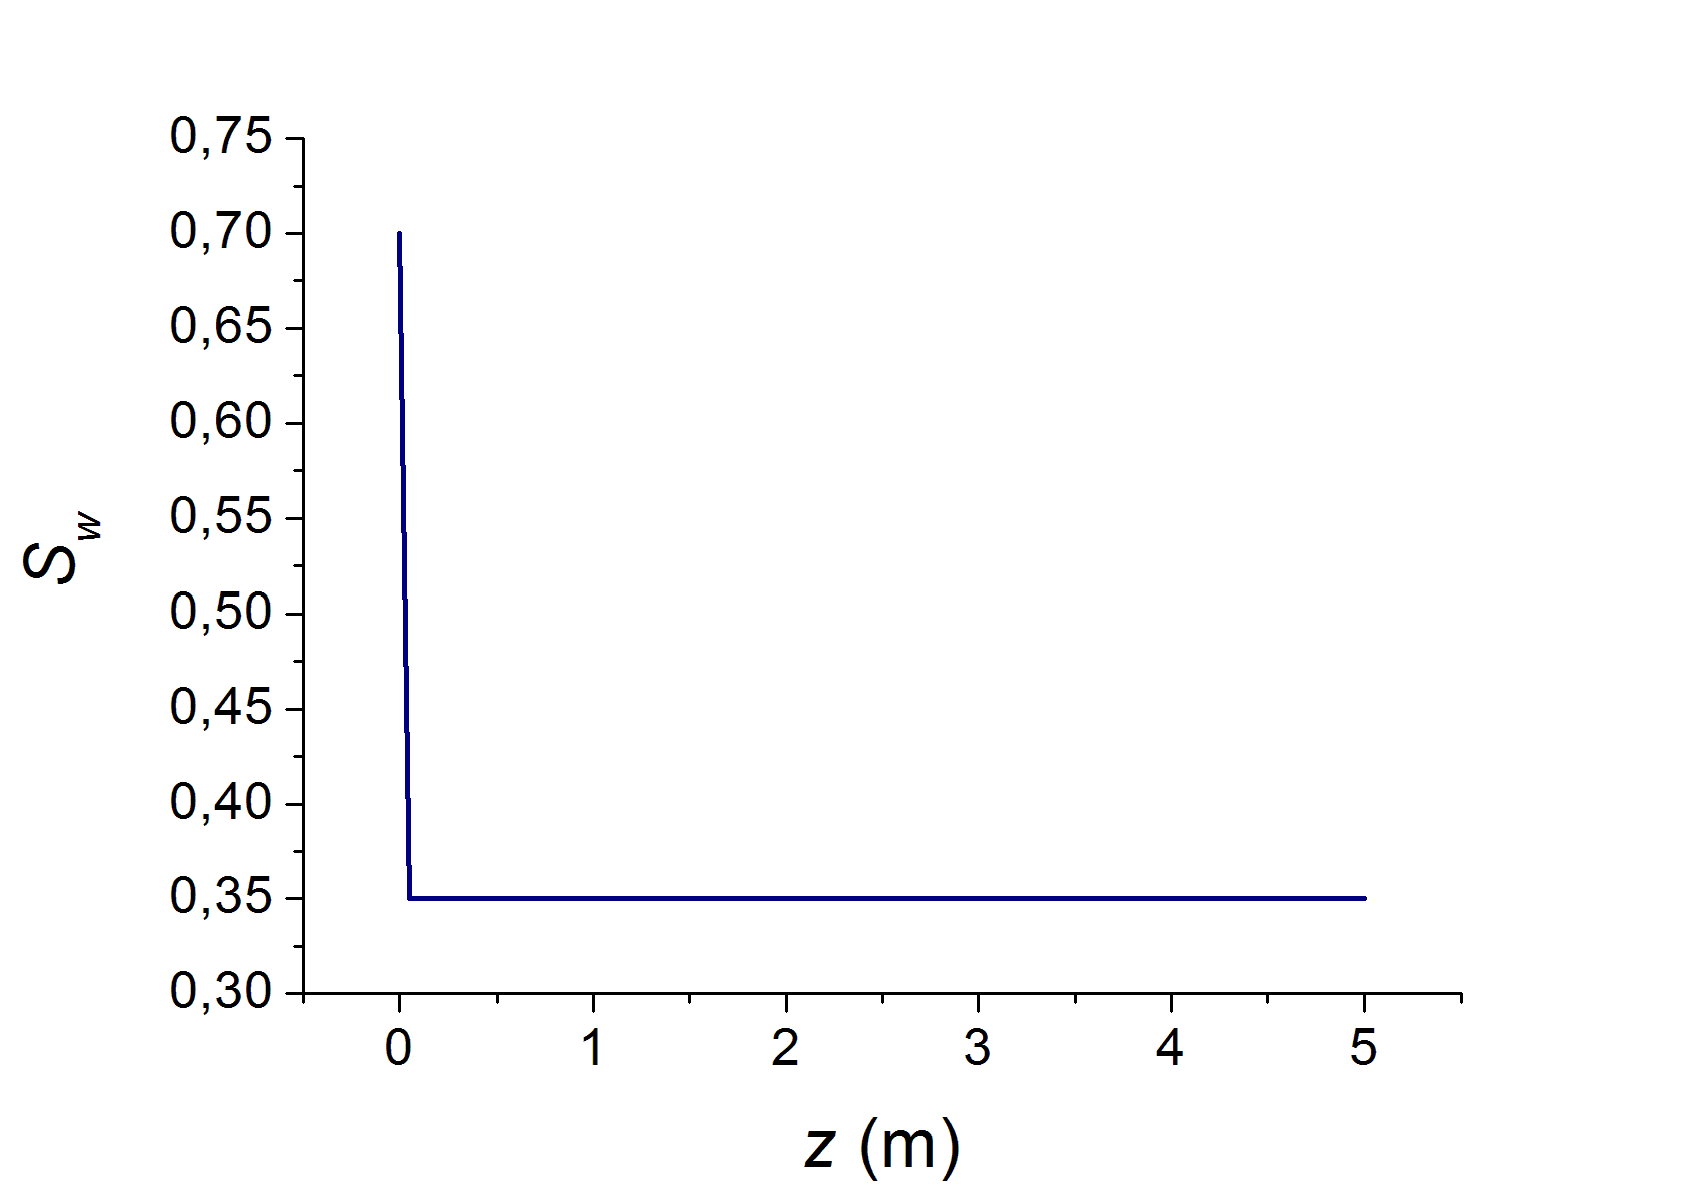
\includegraphics[width=1\textwidth]{test1/init1.png}
       \caption*{Водонасыщенность}
    \end{minipage}
    \hfill
    \begin{minipage}[h]{0.49\textwidth}
       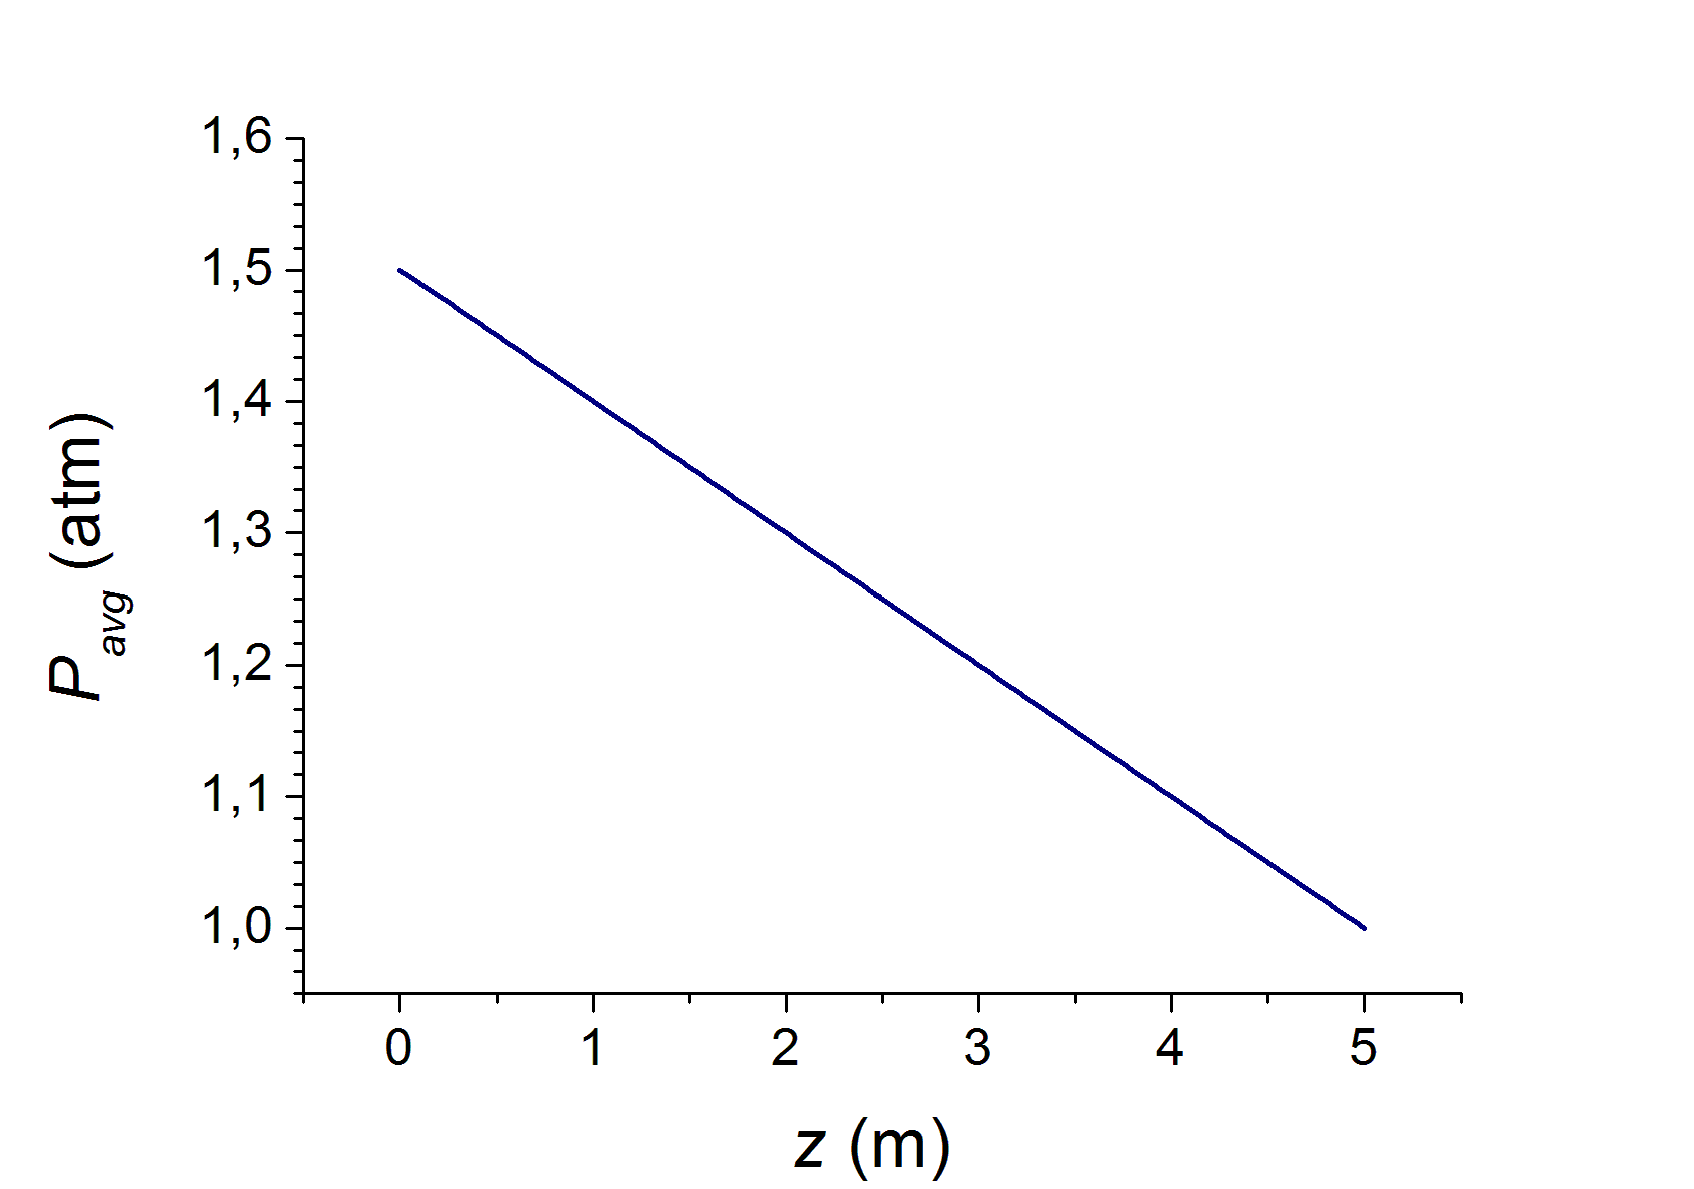
\includegraphics[width=1\textwidth]{test1/init2.png}
       \caption*{Среднее давление}
    \end{minipage}
  \end{center}
  \caption{Распределение водонасыщенности и среднего давления фаз по глубине в начальный момент времени}
  \label{t1_pic1}
\end{figure}

\begin{figure}
  \begin{center}
    \begin{minipage}[h]{0.49\textwidth}
       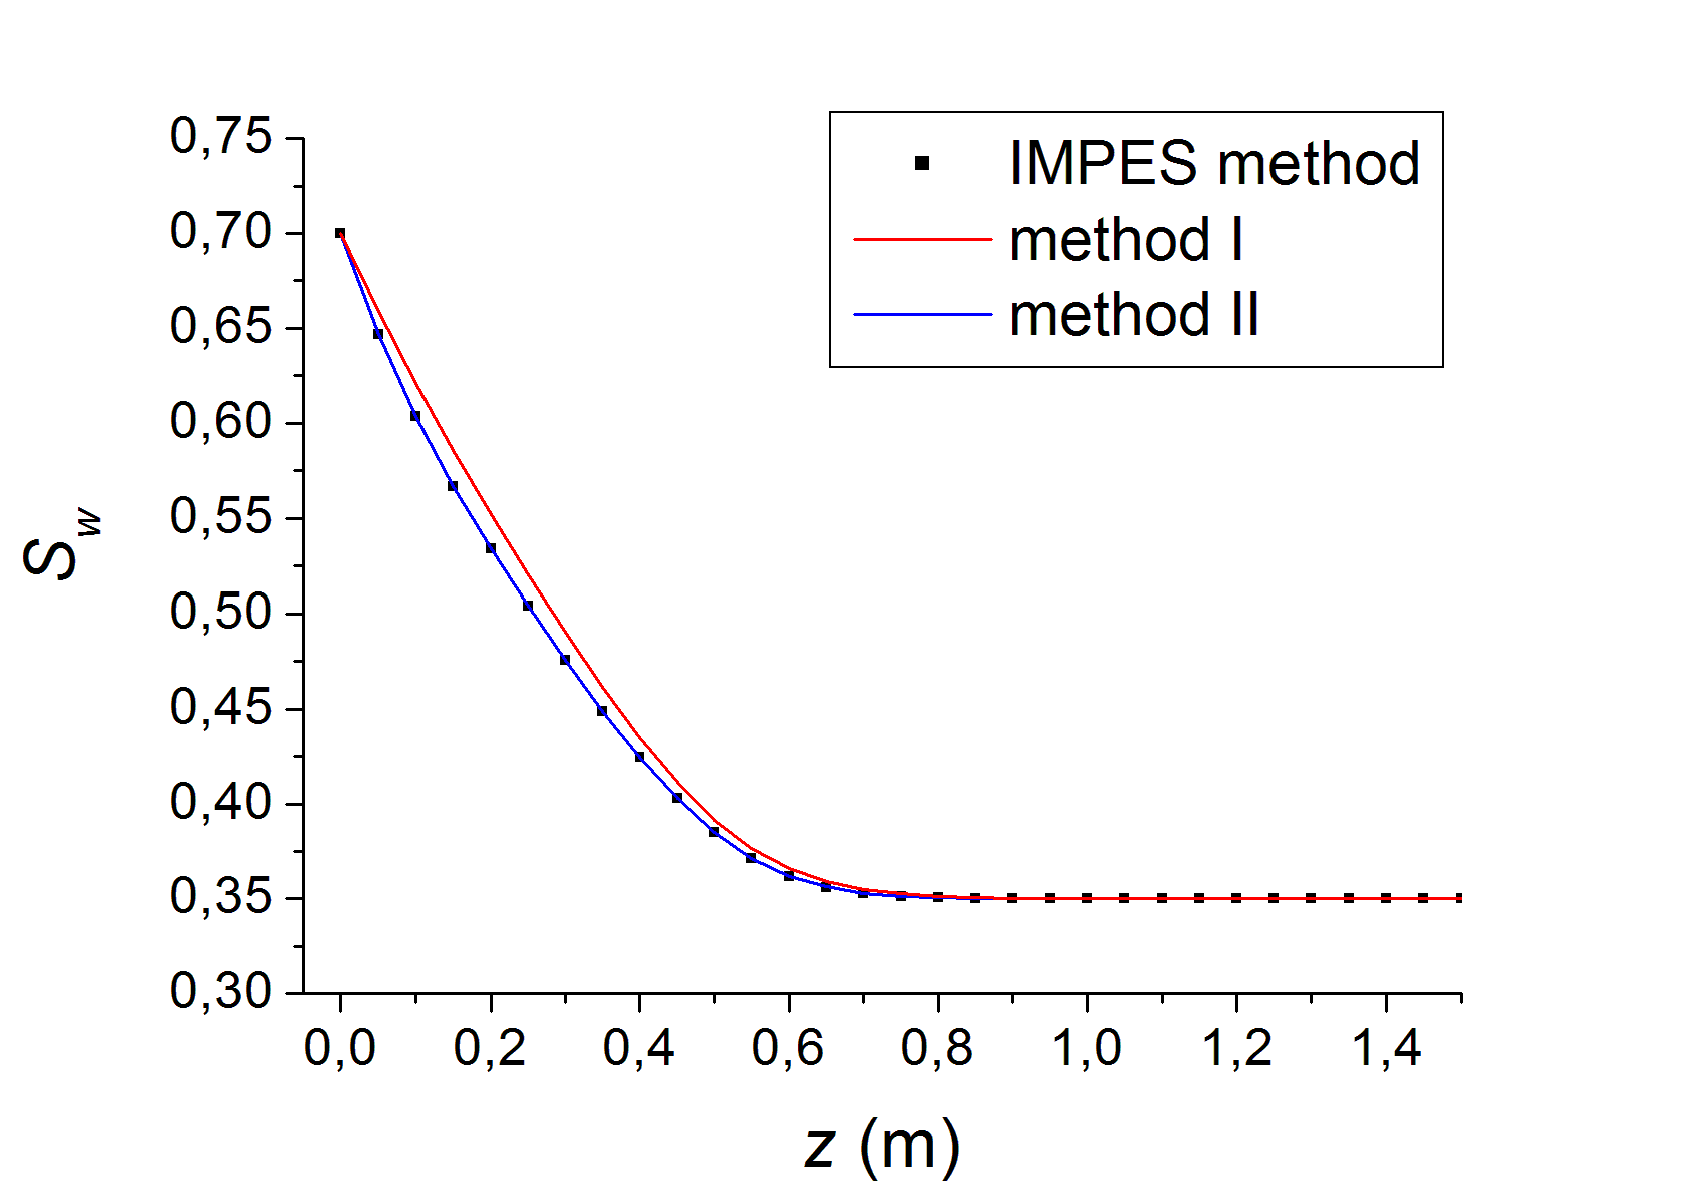
\includegraphics[width=1\textwidth]{test1/res1.png}
       \caption*{Водонасыщенность}
    \end{minipage}
    \hfill
    \begin{minipage}[h]{0.49\textwidth}
       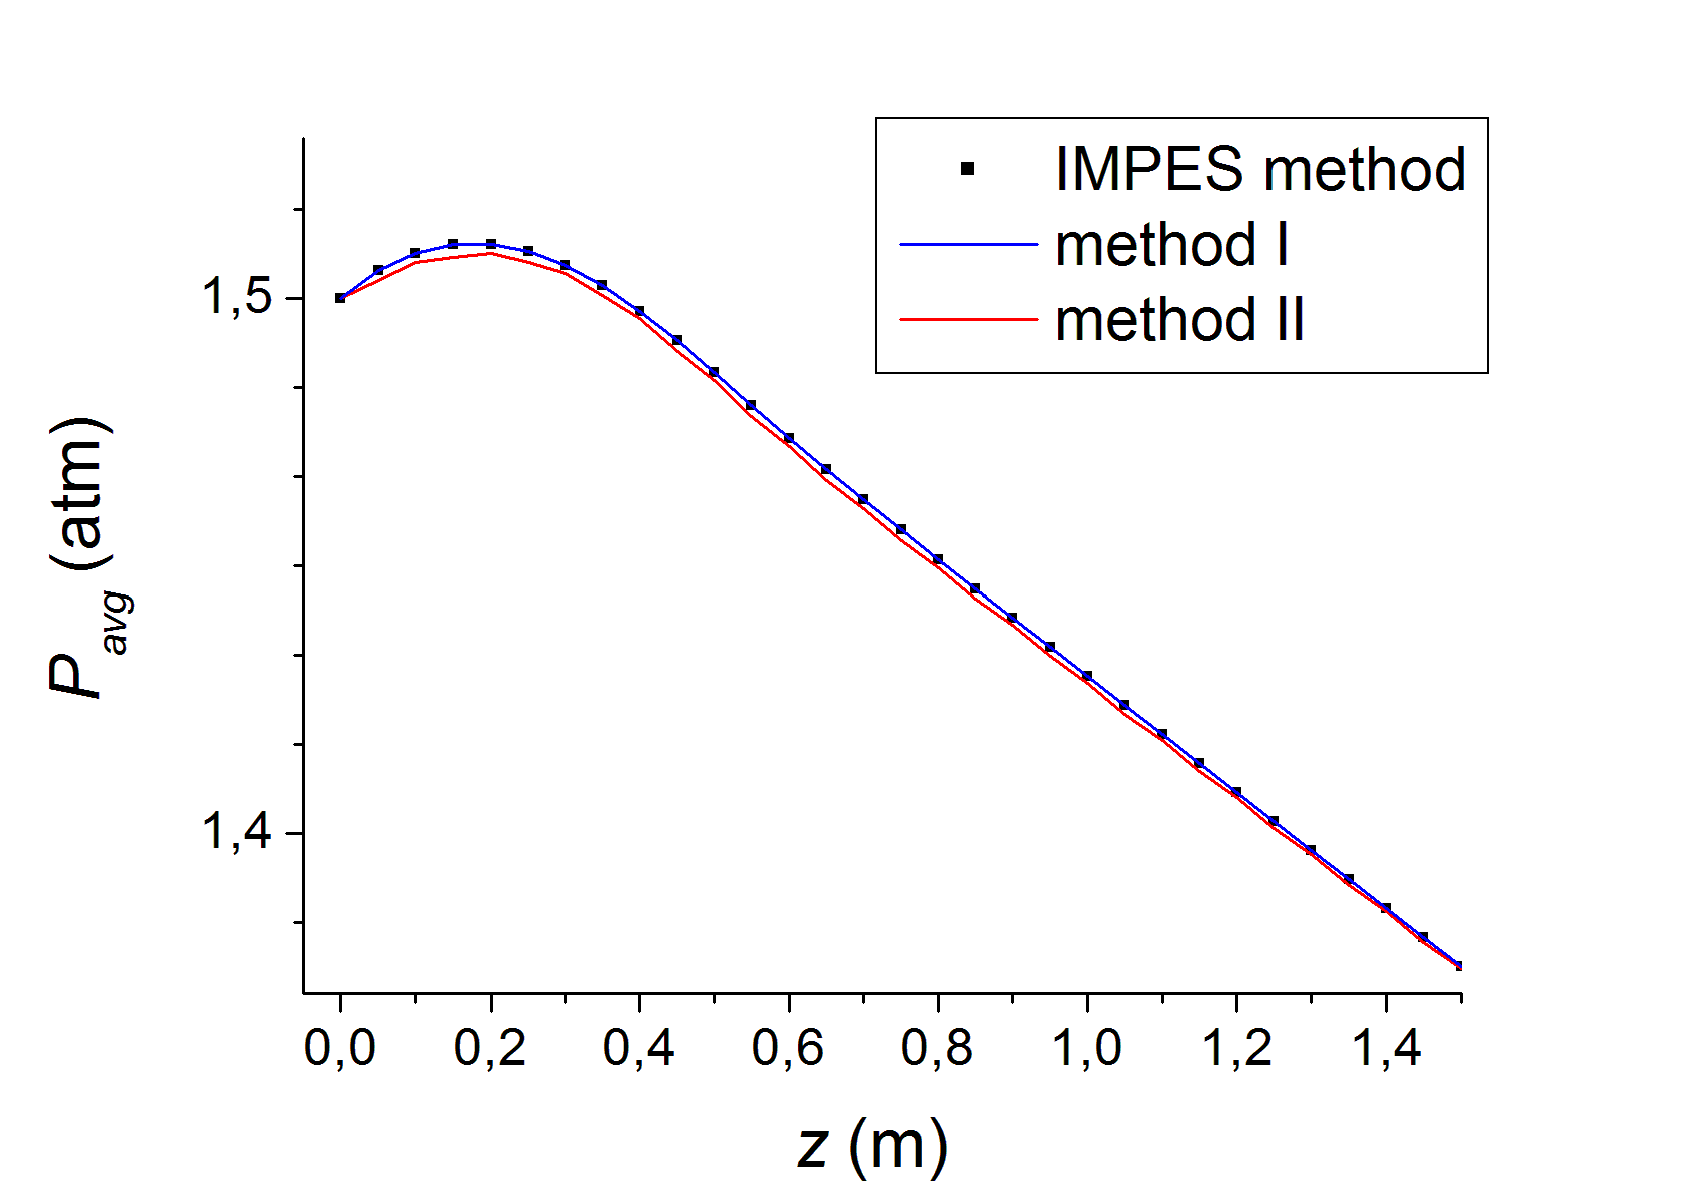
\includegraphics[width=1\textwidth]{test1/res2.png}
       \caption*{Среднее давление}
    \end{minipage}
  \end{center}
  \caption{Распределение водонасыщенности и среднего давления фаз по глубине в момент времени 300c}
  \label{t1_pic2}
\end{figure}

\section{Сравнительный анализ алгоритмов явного типа} \label{ch:ch3/sect2}

Сравним устойчивость двух методов на примере задачи~\ref{ch:ch3/sect1}.
В таблице~\ref{tabular:limits} представлены максимально допустимые для устойчивости временные шаги, экспериментально полученные во время реализации методов I и II. 

\begin{table}[h]
\captionof{table}{Максимальные шаги по времени в алгоритмах на основе гиперболизированных уравнений}
\begin{center}
\begin{tabular}{|c|c|c|}
\hline
\textit {h},м & $\Delta t$,с (метод I) & $\Delta t$,с (метод II) \\
\hline
0.05 & $1.5\dot10^{-3}$ & $3\dot10^{-4}$ \\
\hline
\end{tabular}
\label{tabular:limits}
\end{center}
\end{table}

Для метода I шаг подбирался таким образом, чтобы определитель при обращении матрицы в методе
Ньютона не становился равным нулю. Для метода II шаг выбирался из
условия критического нарастания ошибок, при котором решение <<разваливается>>.
В обоих случаях $\tau=\Delta t$ , то есть значение $\tau$ разное для методов I и II. Варьирование $\tau$ позволяет добиться
повышения $\Delta t$ еще в несколько раз, но не более.
В~\ref{tabular:limits} указан шаг
по времени для метода I больше в несколько раз, чем шаг для метода II, однако
метод I содержит реализацию метода Ньютона в каждом расчетном узле дополнительно по сравнению с явной схемой. По этой причине методы в целом сопоставимыми по вычислительным затратам.

В результате расчетов по методу II было установлено, что учет капиллярного
давления создает необходимость уменьшения шага по времени на порядок. Это можно объяснить сложной зависимостью уравнений для давления и насыщенности от преобладания тех или иных членов, например, при
доминировании капиллярных эффектов поведение решения становится типичным для
параболических уравнений, а ограничение на шаг по времени становится более жестким. 

\section{Трехмерная трехфазная задача просачивания} \label{ch:ch3/sect3}

Исследуемая трехмерная область пористой среды -- куб размера 1м$\times$1м$\times$1м.
Верхняя грань открыта, нижняя -- ограничена резервуаром, через боковые грани
возможно просачивание.
Начальная постановка: вода занимает 10\% области,
нефть и газ распределены по периодическому закону. Ось $y$ направлена вертикально снизу-вверх.
В углу верхней грани расположен источник воды, который занимает девятую часть поверхности. Просачивание происходит под действием силы тяжести. 
Пусть число расчетных узлов -- $N_x\cdot N_y\cdot N_z$.\\
Начальные условия:
\begin{equation}
  \begin{aligned}
    &S_w=0.1,\\
    &S_n(x, y, z)=0.4 + 0.1 \cdot sin^2(x \cdot N_x + y \cdot N_y + z \cdot N_z),\\
    &S_g(x, y, z)=0.4 + 0.1 \cdot cos^2(x \cdot N_x + y \cdot N_y + z \cdot N_z),\\
    &P_w=P_\text{атм}.
   \end{aligned}
\end{equation}
Граничные условия:
\begin{equation}
  \begin{aligned}
    &\left.P\right|_{y=1,\ 0 < x < 0.33,\ 0 < z < 0.33}=P_{\text{атм}},\\
    &\left.{P_i}\right|_{y=0}\text{ определяется из условия } \left.(\overrightarrow{u_i} \cdot \overrightarrow{n})\right|_{y=0}=0;\\
    &\left.S_w\right|_{y=1,\ 0 < x < 0.33,\ 0 < z < 0.33}=0.6,\\
    &\left.S_n\right|_{y=1,\ 0 < x < 0.33,\ 0 < z < 0.33}=0.05,\\
    &\text{на остальных граничных поверхностях потоки}\\
    &S_w,\ S_n,\ P_w\ \text{эквиваленты нулю по направлению нормали.}
  \end{aligned}
\end{equation}

На ~\ref{t4_pic_start}-~\ref{t4_pic_end} проиллюстрированы результаты вычислений, приведены распределения давления,
и~насыщенностей водной и нефтяной фаз в три различные момента времени. Видно распространение фронтов от источника по области, вблизи нижней границы вода накопливается и постепенно вытесняет другие фазы через верхнюю и боковые грани.

\begin{figure}
  \begin{center}
    \begin{minipage}[h]{0.49\textwidth}
       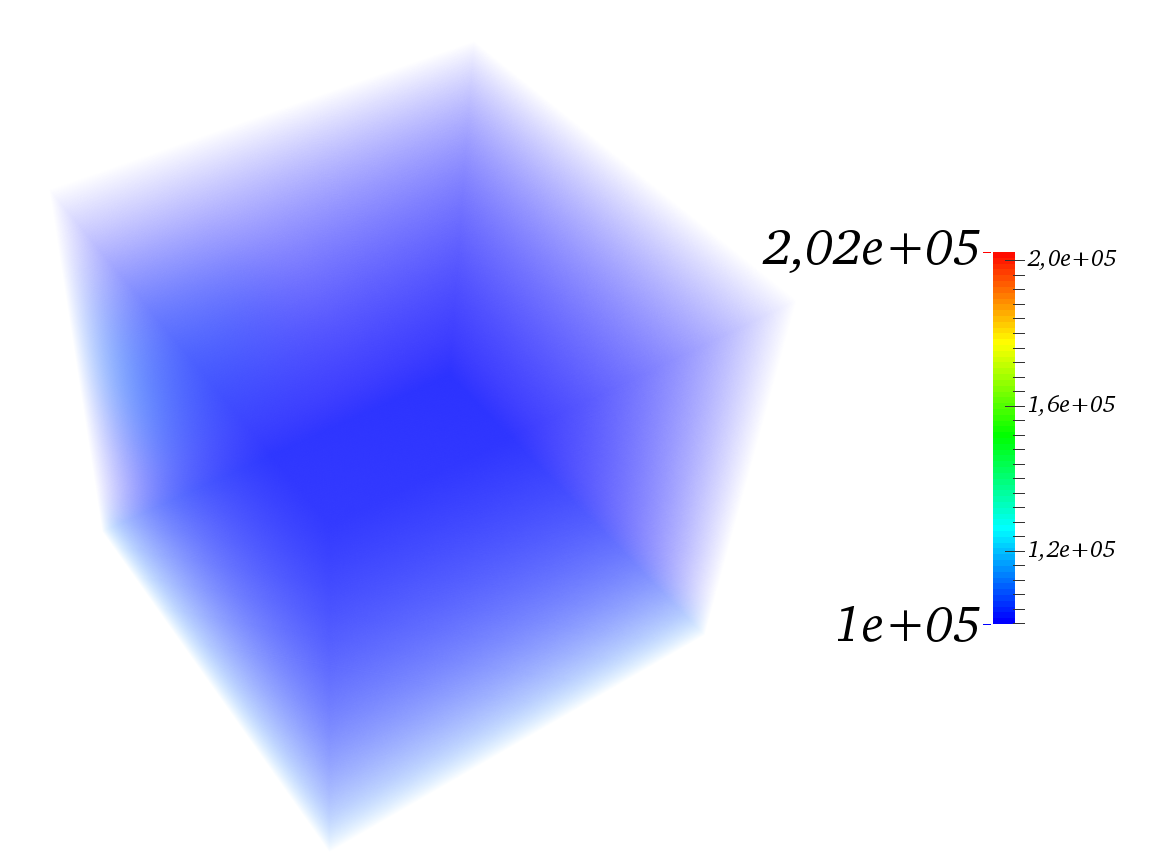
\includegraphics[width=1\textwidth]{test4/pw_200.png}
       \vspace{1cm}
       \caption{Давление $P_w$ в момент времени $t=200$с}
       \label{t4_pic_start}
    \end{minipage}
    \hfill
    \begin{minipage}[h]{0.49\textwidth}
       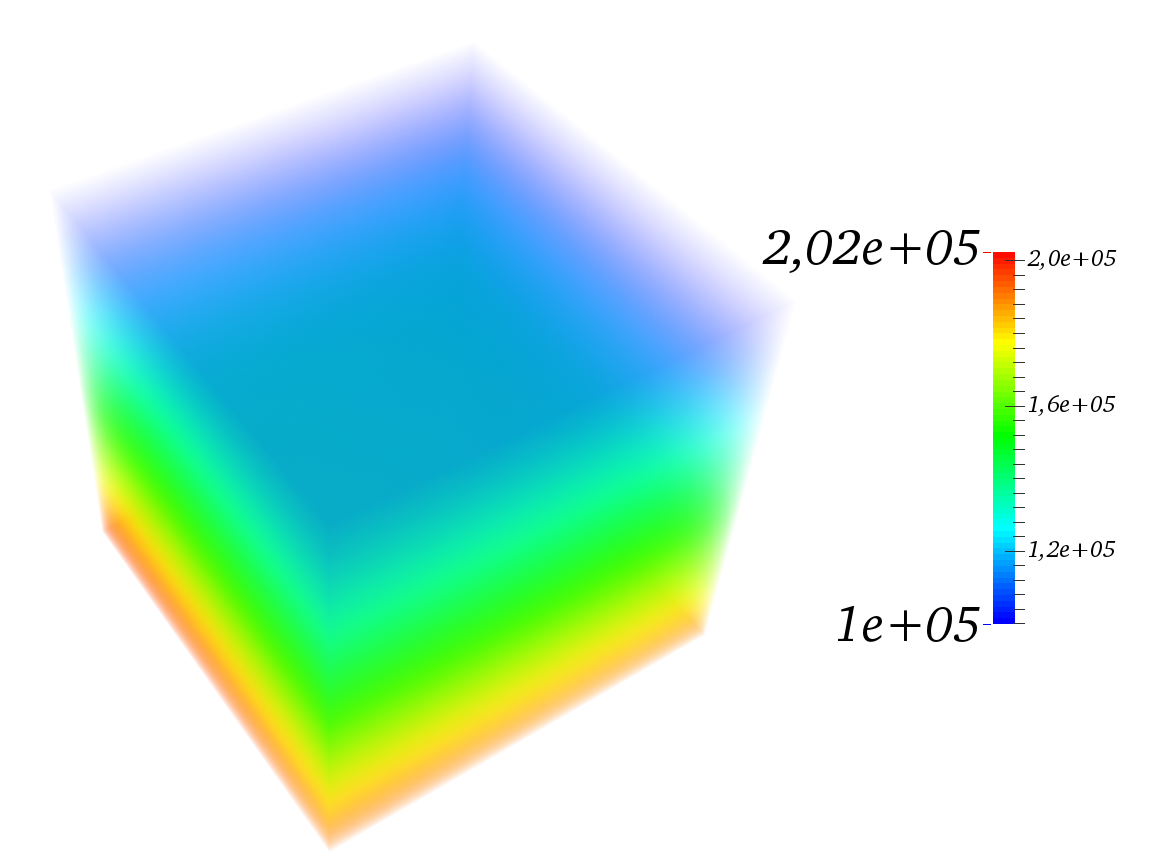
\includegraphics[width=1\textwidth]{test4/pw_1000.png}
       \vspace{1cm}
       \caption{Давление $P_w$ в момент времени $t=1000$с}
    \end{minipage}
    \vspace{3cm}
    \vfill
    \begin{minipage}[h]{0.49\textwidth}
       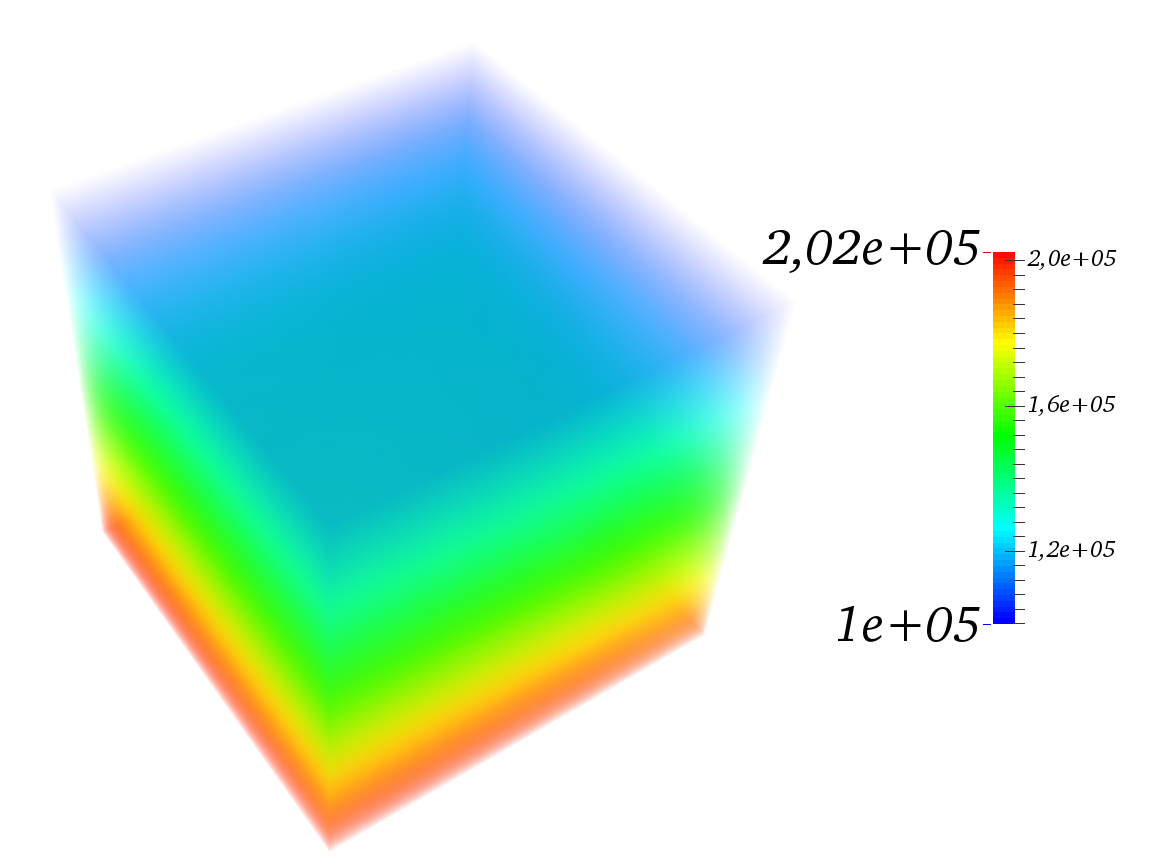
\includegraphics[width=1\textwidth]{test4/pw_2000.png}
       \vspace{1cm}
       \caption{Давление $P_w$ в момент времени $t=2000$с}
    \end{minipage}
    \hfill
    \begin{minipage}[h]{0.49\textwidth}
       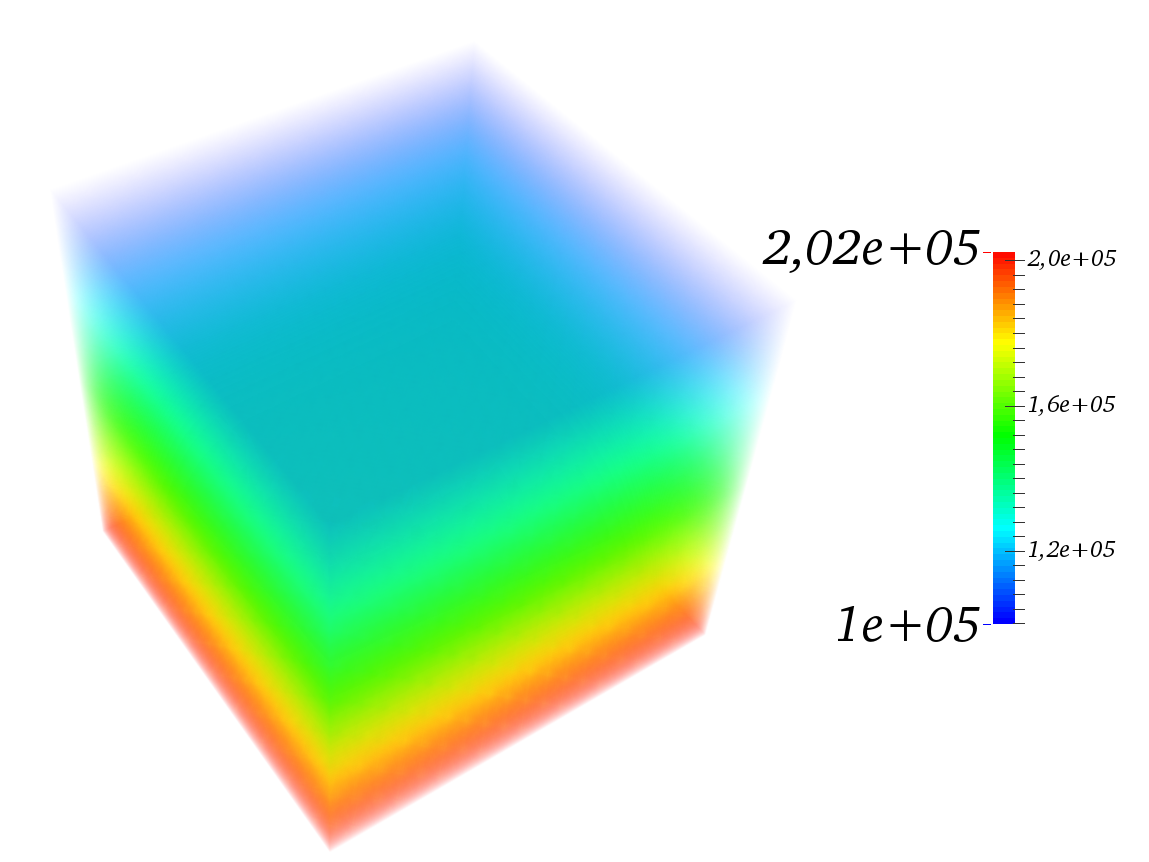
\includegraphics[width=1\textwidth]{test4/pw_6600.png}
       \vspace{1cm}
       \caption{Давление $P_w$ в момент времени $t=6600$с}
    \end{minipage}
    \hfill  
  \end{center}
\end{figure}

\begin{figure}
  \begin{center}
    \begin{minipage}[h]{0.49\textwidth}
       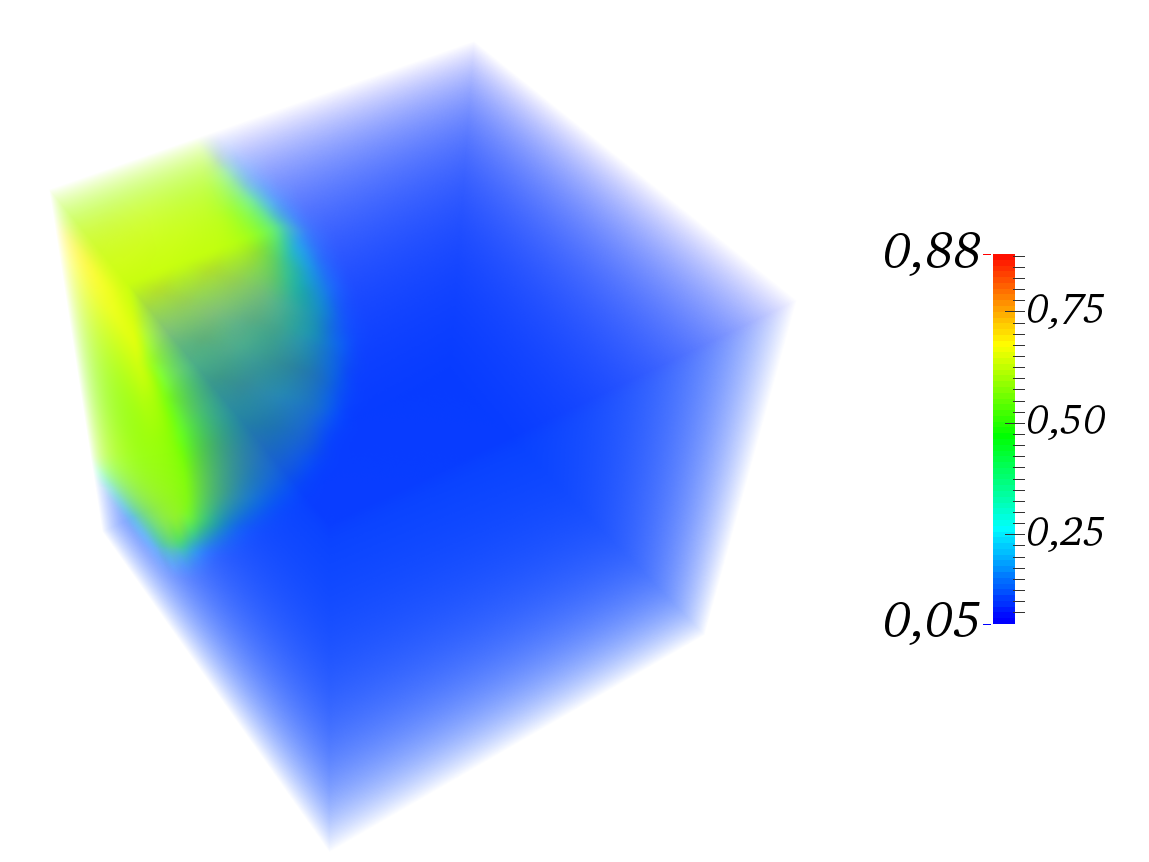
\includegraphics[width=1\textwidth]{test4/sw_200.png}
       \vspace{1cm}
       \caption{Насыщенность $S_w$ в момент времени $t=200$с}
    \end{minipage}
    \hfill
    \begin{minipage}[h]{0.49\textwidth}
       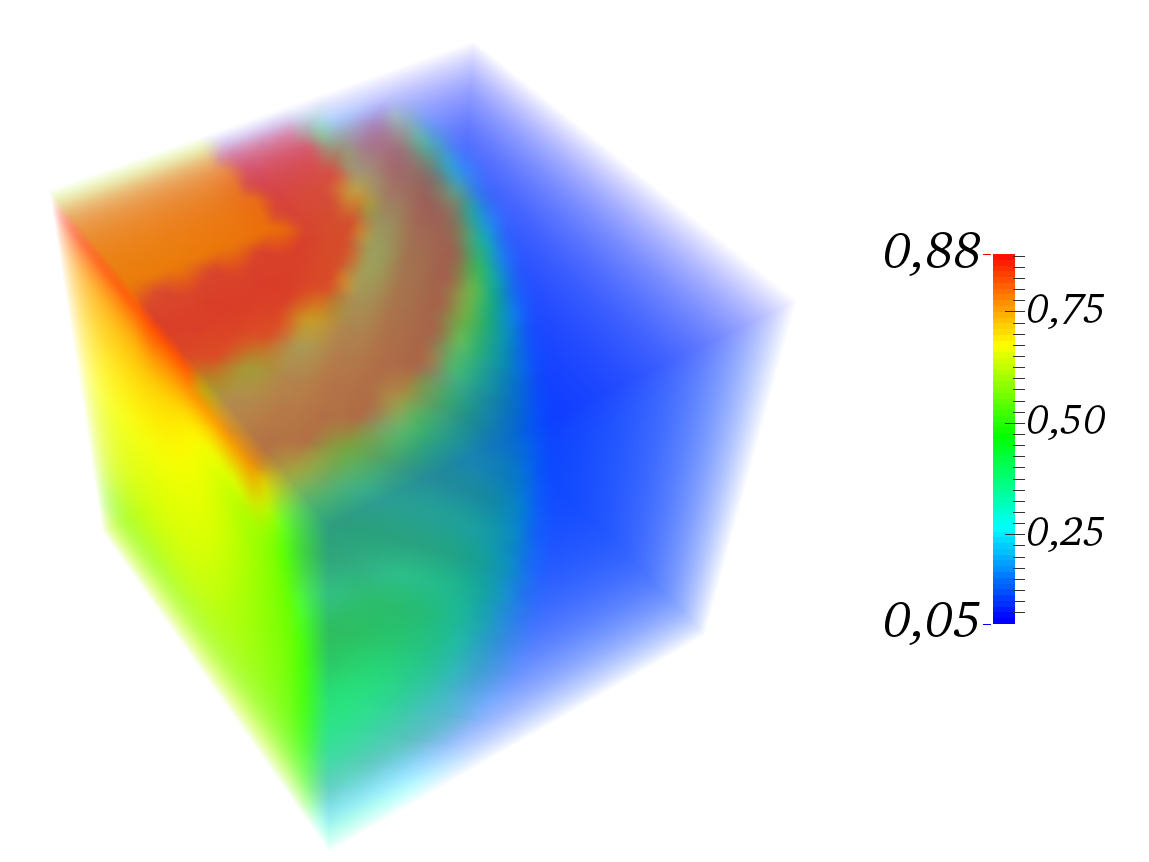
\includegraphics[width=1\textwidth]{test4/sw_1000.png}
       \vspace{1cm}
       \caption{Насыщенность $S_w$ в момент времени $t=1000$с}
    \end{minipage}
    \vspace{3cm}
    \vfill
    \begin{minipage}[h]{0.49\textwidth}
       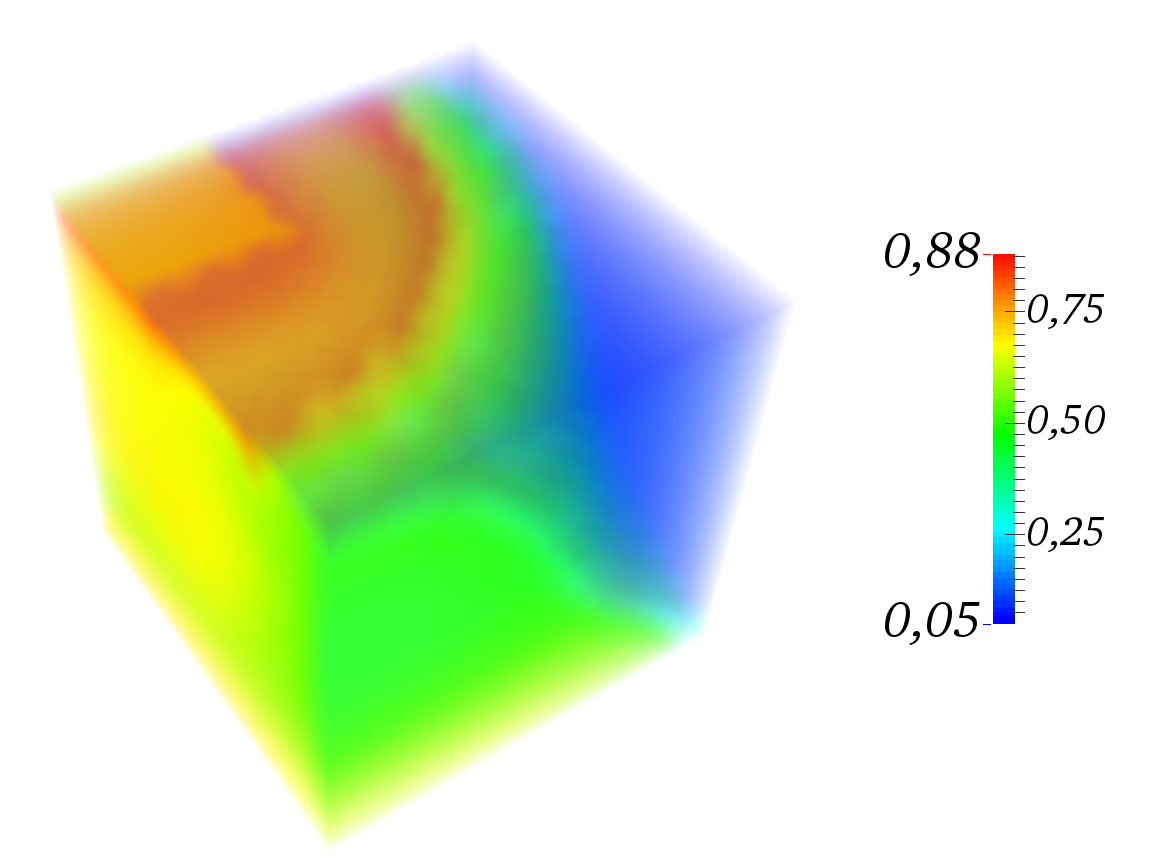
\includegraphics[width=1\textwidth]{test4/sw_2000.png}
       \vspace{1cm}
       \caption{Насыщенность $S_w$ в момент времени $t=2000$с}
    \end{minipage}
    \hfill
    \begin{minipage}[h]{0.49\textwidth}
       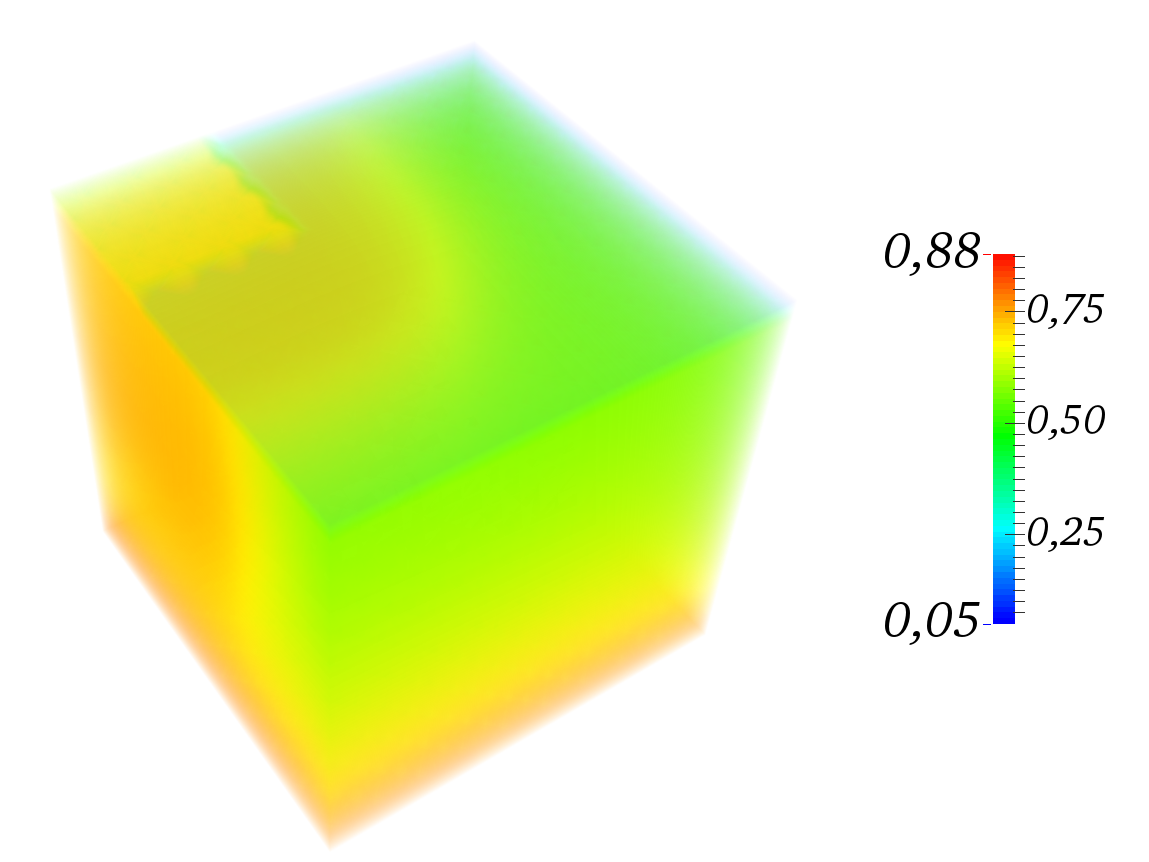
\includegraphics[width=1\textwidth]{test4/sw_6600.png}
       \vspace{1cm}
       \caption{Насыщенность $S_w$ в момент времени $t=6600$с}
    \end{minipage}
    \hfill  
  \end{center}
\end{figure}

\begin{figure}
  \begin{center}
    \begin{minipage}[h]{0.49\textwidth}
       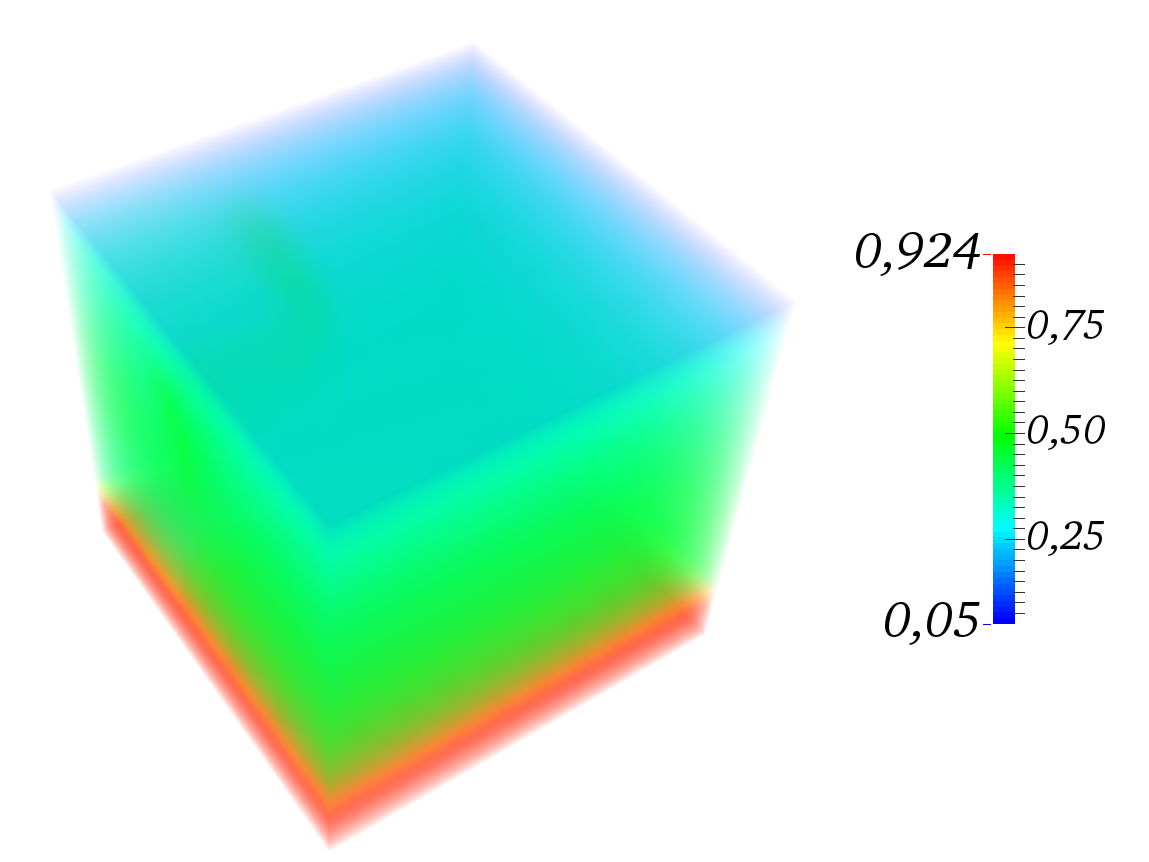
\includegraphics[width=1\textwidth]{test4/sn_200.png}
       \vspace{1cm}
       \caption{Насыщенность $S_n$ в момент времени $t=200$с}
    \end{minipage}
    \hfill
    \begin{minipage}[h]{0.49\textwidth}
       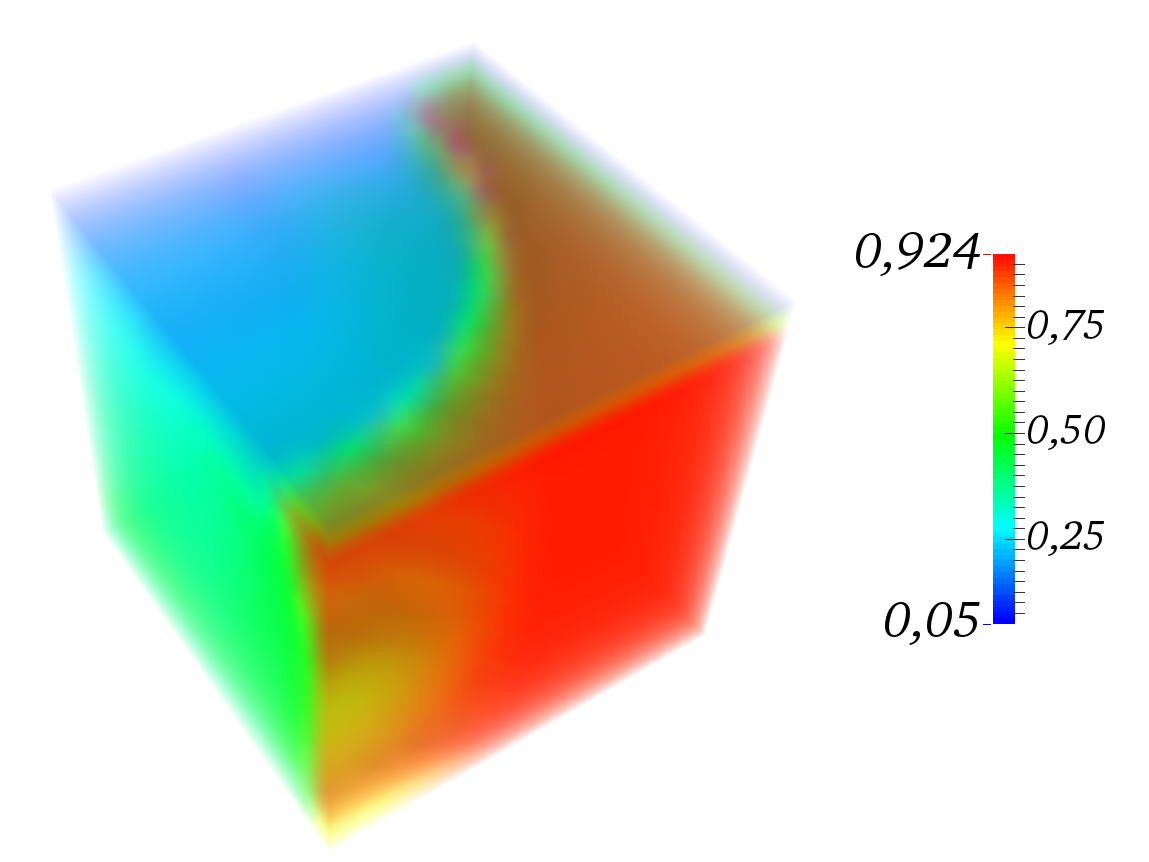
\includegraphics[width=1\textwidth]{test4/sn_1000.png}
       \vspace{1cm}
       \caption{Насыщенность $S_n$ в момент времени $t=1000$с}
    \end{minipage}
    \vspace{3cm}
    \vfill
    \begin{minipage}[h]{0.49\textwidth}
       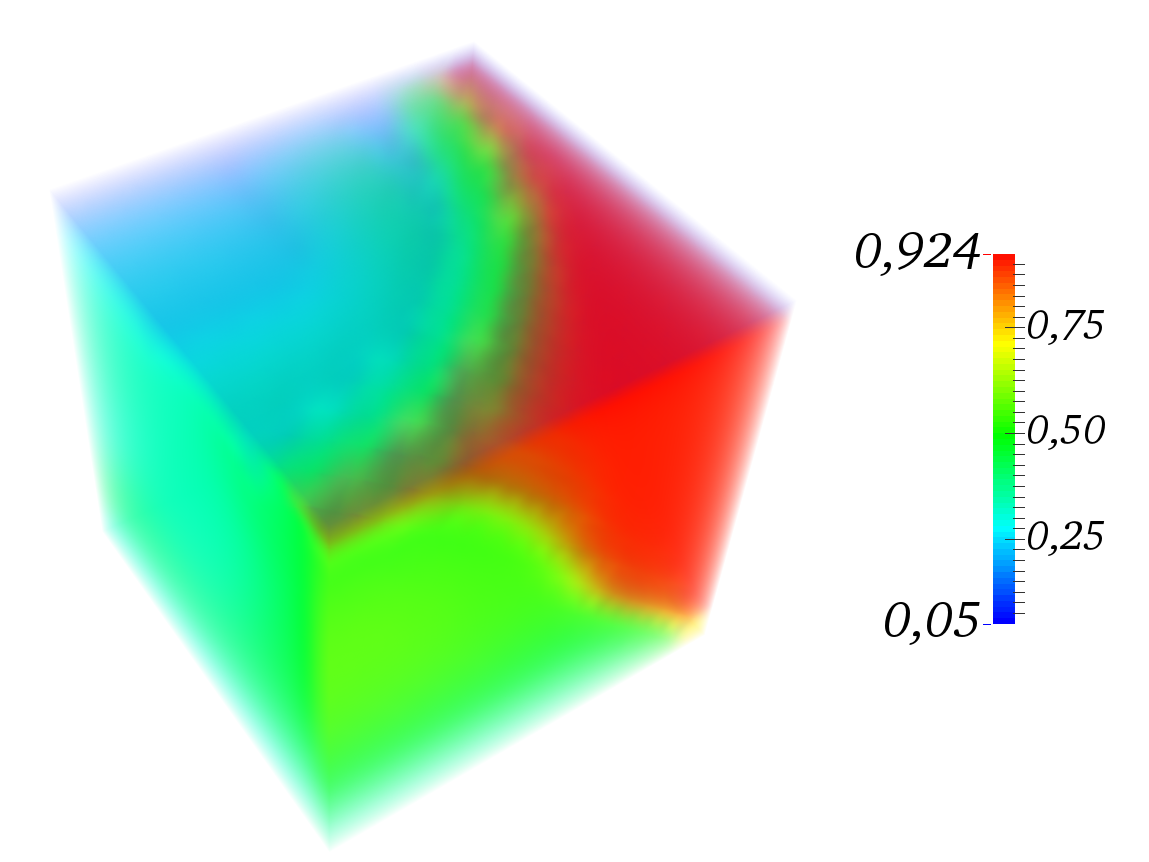
\includegraphics[width=1\textwidth]{test4/sn_2000.png}
       \vspace{1cm}
       \caption{Насыщенность $S_n$ в момент времени $t=2000$с}
    \end{minipage}
    \hfill
    \begin{minipage}[h]{0.49\textwidth}
       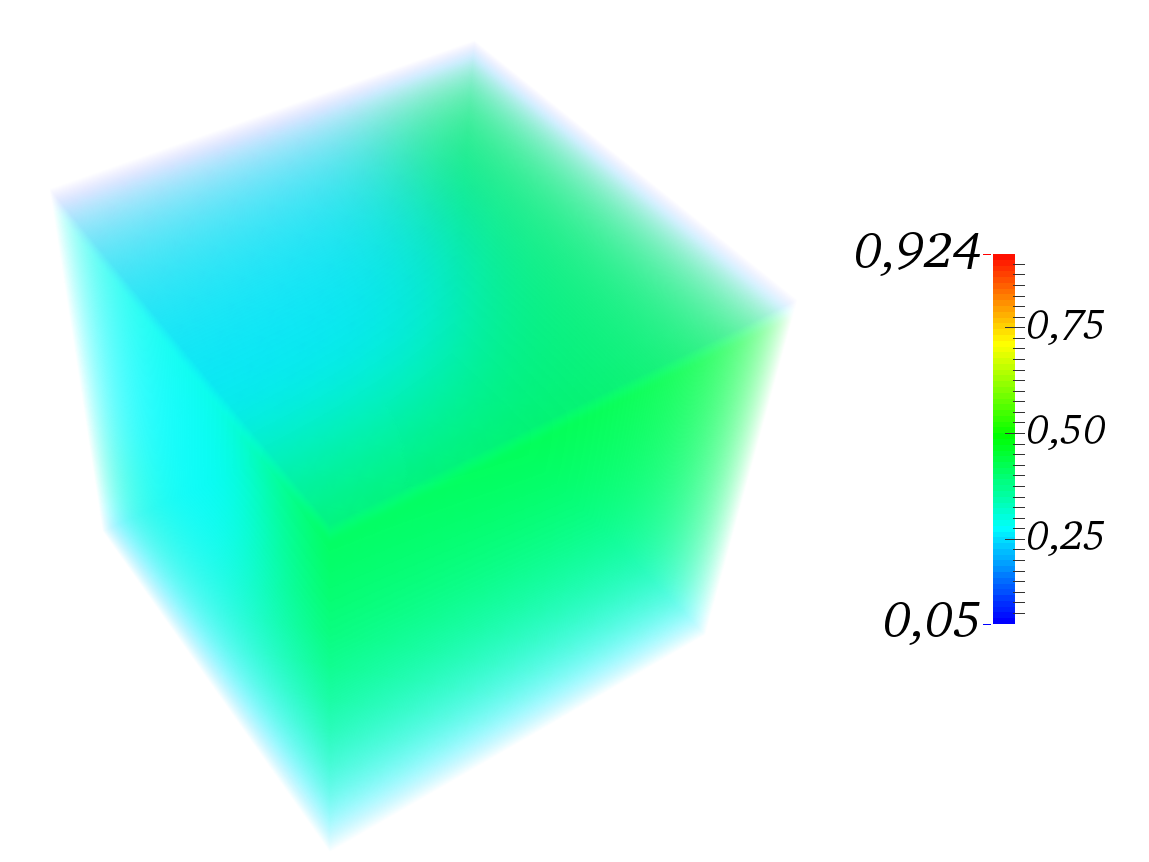
\includegraphics[width=1\textwidth]{test4/sn_6600.png}
       \vspace{1cm}
       \caption{Насыщенность $S_n$ в момент времени $t=6600$с}
       \label{t4_pic_end}
    \end{minipage}
    \hfill  
  \end{center}
\end{figure}
           % Глава 3
\chapter{Использование высокопроизводительных вычислительных систем} \label{ch:ch4}

В данной работе рассматривается применение технологии программно-аппаратной архитектуры параллельных вычислений CUDA, позволяющей производить вычисления на графических процессорах (GPU), к задачам трехфазной фильтрации.
Портирование кода происходило на базе примеров из ~\cite{Sanders-CUDA}.
Также реализована возможность многопроцессорных вычислений с использованием
интерфейса передачи сообщений MPI.

\section{Практические аспекты программной реализации} \label{ch:ch4/sect1}

В работе представлен гибкий и хорошо масштабируемый механизм разделения
расчетной сетки на локальные подсетки. Благодаря такому механизму
нет необходимости хранить расчетную сетку целиком на каком-либо из
процессоров, а преобразование локальных координат в глобальные
позволяет воссоздать общую картину полученных в результате расчетов
данных. Для однородности способа обращения к данным независимо
от размерности задачи используется одномерная индексация массивов.

Параллельной реализация основана на принципе геометрического параллелизма.
Возможно деление области на подобласти как в~одном, так и двух или трех направлениях.
Перед непосредственным стартом вычислений оцениваем с помощью разработанного алгоритма расчетное время в зависимости от разбиения
области, выясняем, какой способ деления области предпочтительнее и эффективнее в точки зрения распределения нагрузки между вычислительными узлами.
Можно сказать, что процесоры образуют сетку, в~которой местоположение каждого процессора может быть задано с~помощью декартовых координат.

Для лучшей масштабируемости системы, удобства визуализации и обращения
к данным ведется запись результатов расчетов всеми процессорами в один большой файл -- каждый процессор
пишет свой фрагмент этого файла. Реализован механизм синхронизации доступа к файлу.

\section{Результаты расчетов на суперкомпьютере} \label{ch:ch4/sect2}

Большая часть расчетов проводилась на гибридном вычислительном кластере К-100, расположенном в ИПМ им. М.В.Келдыша РАН.
Ускорения и эффективность вычислений были проанализированы на примере трехмерной тестовой задачи~\ref{ch:ch3/sect3}.
Время расчета измерялось с помощью счетчика, встроенного в программный код.

Исследуем ускорения и эффективности вычислений в зависимости от числа
используемых для расчета процессоров. Результаты измерений приведены
на графиках (Рис.~\ref{mpi_speedup}, Рис.~\ref{mpi_eff}).
Измерялось время расчета 50 шагов по времени на сетке размером 4 миллиона узлов.
Ступенчатая структура ускорений и, следовательно, скачки эффективности наблюдаются
в связи с неодинаковым способом распределения нагрузки между процессорами
в зависимости от их числа, а также погрешностью вычислений. Сохранение высокой
эффективности вычислений (84-95\%) обусловлено значительным превосходством времени, требуемого
непосредственно для расчета, по~сравнению с временем, необходимым для обмена данными
между процессорами.

\begin{figure}[!h]
\begin{center}
\begin{tikzpicture}
  \begin{axis}[axis lines=left, enlargelimits=true, grid=major, width=0.7\textwidth, xlabel={\textit{число процессоров}}, ylabel={\textit{ускорение}}]
    \pgfplotstableread{data/mpi_times.txt}{\mytable}
    \pgfplotstablegetelem{0}{Y}\of{\mytable}
    \pgfmathsetmacro{\ay}{\pgfplotsretval}
    \addplot [blue, mark=*] table [x=X, y expr=\ay/\thisrow{Y}] {\mytable};
  \end{axis}
\end{tikzpicture}
\caption{Зависимость ускорения расчета тестовой задачи от числа процессоров}
\label{mpi_speedup}
\end{center}
\end{figure}

\begin{figure}[!h]
\begin{center}
\begin{tikzpicture}
  \begin{axis}[axis lines=left, enlargelimits=true, grid=major, width=0.7\textwidth, xlabel={\textit{число процессоров}}, ylabel={\textit{эффективность}}]
    \pgfplotstableread{data/mpi_times.txt}{\mytable}
    \pgfplotstablegetelem{0}{Y}\of{\mytable}
    \pgfmathsetmacro{\ay}{\pgfplotsretval}
    \addplot [blue,mark=*] table [x=X, y expr=\ay/\thisrow{Y}/\thisrow{X}] {\mytable};
  \end{axis}
\end{tikzpicture}
\caption{Зависимость эффективности расчета тестовой задачи от числа процессоров}
\label{mpi_eff}
\end{center}
\end{figure}

Рассмотрим, как меняется время решения поставленной задачи при~проведении расчетов на~GPU
с~помощью CUDA. На~Рис.~\ref{cuda_speedup} изображена зависимость укорения тестового расчета на~одном GPU
по~сравнению с~одним CPU. Измерения проводились для~различного числа
узлов расчетной сетки. Как видно из~приведенного на~Рис.~\ref{cuda_speedup}
графика, для~сеток малого размера (8000 узлов) возможно замедление расчетов, но~при~увеличении
размера сетки наблюдается все большее ускорение расчета. При~этом для~большей из~
рассмотренных сеток (2.2 миллиона узлов) полученное ускорение составило 3.5 раза.

\begin{figure}[!h]
\begin{center}
\begin{tikzpicture}
  \begin{axis}[axis lines=left, enlargelimits=true, grid=major, width=0.7\textwidth, xlabel={\textit{число узлов сетки}}, ylabel={\textit{ускорение}}]
    \pgfplotstableread[skip first n=1]{data/cpu_vs_gpu.txt}{\mytable}
    \addplot [blue, mark=*] table [x=0, y expr=\thisrow{1}/\thisrow{2}] {\mytable};
  \end{axis}
\end{tikzpicture}
\caption{Зависимость ускорения расчета тестовой задачи от числа узлов расчетной сетки на одном GPU по сравнению с одним CPU}
\label{cuda_speedup}
\end{center}
\end{figure}

Следует отметить, что~эффективное использование больших вычислительных
мощностей является трудоемкой задачей и~требует глубокого исследования и~понимания
архитектуры вычислительных систем.
           % Глава 4
\chapter*{Заключение}                       % Заголовок
\addcontentsline{toc}{chapter}{Заключение}  % Добавляем его в оглавление

%% Согласно ГОСТ Р 7.0.11-2011:
%% 5.3.3 В заключении диссертации излагают итоги выполненного исследования, рекомендации, перспективы дальнейшей разработки темы.
%% 9.2.3 В заключении автореферата диссертации излагают итоги данного исследования, рекомендации и перспективы дальнейшей разработки темы.
%% Поэтому имеет смысл сделать эту часть общей и загрузить из одного файла в автореферат и в диссертацию:

Основные результаты работы заключаются в следующем:
\begin{enumerate}
 \item Выведены гиперболизированные системы уравнений фильтрации двумя способами;
 \item Аппроксимированы уравнения явными разностыми схемами;
 \item Разработаны алгоритмы решения полученных систем уравнений;
 \item Разработан комплекс программ для проведения вычислений, ориентированный на использование суперкомпьютеров;
 \item Проведены вычислительные эксперименты;
 \item Проведены сравнения решений известных тестовых задач о просачивании многофазных жидкостей в пористых средах под действием силы тяжести или заданного градиента давления с IMPES-методом и решениями других авторов.
\end{enumerate}

Результаты тестовых расчетов показали, что использование предложенной модификацированной модели и явной позволяет существенно увеличить шаг по времени как минимум на порядок, а значит ускорить численное решение. Кроме того, явные схемы позволяют более эффективно применять параллельные вычисления.
При этом качественный характер течений не меняется, а погрешность вычислений остается приемлемой.

Данная тема в дальнейшем может быть разработана путем учета ряда дополнительных физических явлений, а также обобщения на случай течений многокомпонентных многофазных жидкостей в пористых средах.
      % Заключение

%\nocite{*}
\bibliographystyle{biblio/utf8gost705u}
\bibliography{biblio/external}
\newpage
\addcontentsline{toc}{chapter}{Список публикаций}
\renewcommand{\bibsection}{\chapter*{Список публикаций}}
\nociteauthor{*}
\bibliographystyleauthor{biblio/utf8gost71u}
\bibliographyauthor{biblio/author}

\end{document}
